\documentclass[english]{amsart}
\usepackage{geometry}
\geometry{verbose,tmargin=1in,bmargin=1in,lmargin=1in,rmargin=1in}
%\usepackage{fancyhdr}
%\pagestyle{fancy}
\setlength{\parskip}{\smallskipamount}
\setlength{\parindent}{0pt}
\usepackage{amsthm}
\usepackage{amsmath}
\usepackage{graphicx}
\usepackage{hyperref}
\usepackage{caption}
\usepackage{fancyhdr}
\usepackage{subcaption}
\usepackage{float}
\usepackage[authoryear]{natbib}
\DeclareMathOperator*{\argmax}{arg\,max}
\usepackage{graphicx}
\graphicspath{{../figures/}}

\begin{document}

\title{STAT 215A --- FMRI data decoding}

\author{Xiang Li}

\maketitle

\section{Introduction}
The human brain processes a dizzying array of electromagnetic radiation into a coherent {\it picture} of the world. How it does so is a fascinating scientific question.  After all, the bounty of visual metaphors that pervade thought and speech is a clear reminder of the integral part vision plays in cognition.  In this lab, armed with some FMRI data collected by the Gallant lab, we build and analyze predictive models for brain response to natural pictures, and study these models to inform the scientific question of how we process visual information, with the goal of decoding brain responses back to visual data. 

\section{Data}
The response dataset was collected by an FMRI machine, which measures the intensity of blood flow to regions of the brain.  The degree of resolution of these measurements are $2mm \times 2mm \times 4mm$ regions called voxels.  The subject was shown thousands of natural images (1750 of which are provided for the training set of this lab and 120 for testing) and the intensity of blood flow was recorded for each voxel as a vector of response, of length the number of pictures.  FMRI data is riddled with noise, and the dataset was already preprocessed in many ways, such as decorrelating voxel intensities with ambient intensities (periodic or random) across the brain. \\

Our dataset is restricted to the responses of 20 voxels, all located in what is denoted the $V1$ processing center of the brain.  V1 is regarded as the first processing center, and many papers suggest that our brain at this level does a Gabor wavelet like transformation.  This is motivation for the initial transformation of the feature set, given by $120 \times 120$ pixel intensities of a grayscale image, using Gabor wavelets.  This transformation is essentially a localized complex Fourier transforms of the $120 \times 120$ dimensional space.  Our data matrix is thus a matrix of the coefficients of the basis of wavelets.

\section{EDA}

\begin{figure}[H]
\minipage{0.28\textwidth}
  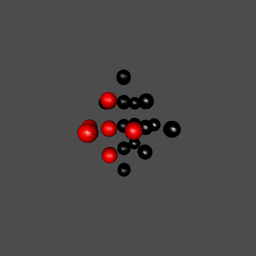
\includegraphics[width=\linewidth, height = 100pts]{voxel_plot.png}
\endminipage\hfill
\vspace{-5mm}
\minipage{0.33\textwidth}
  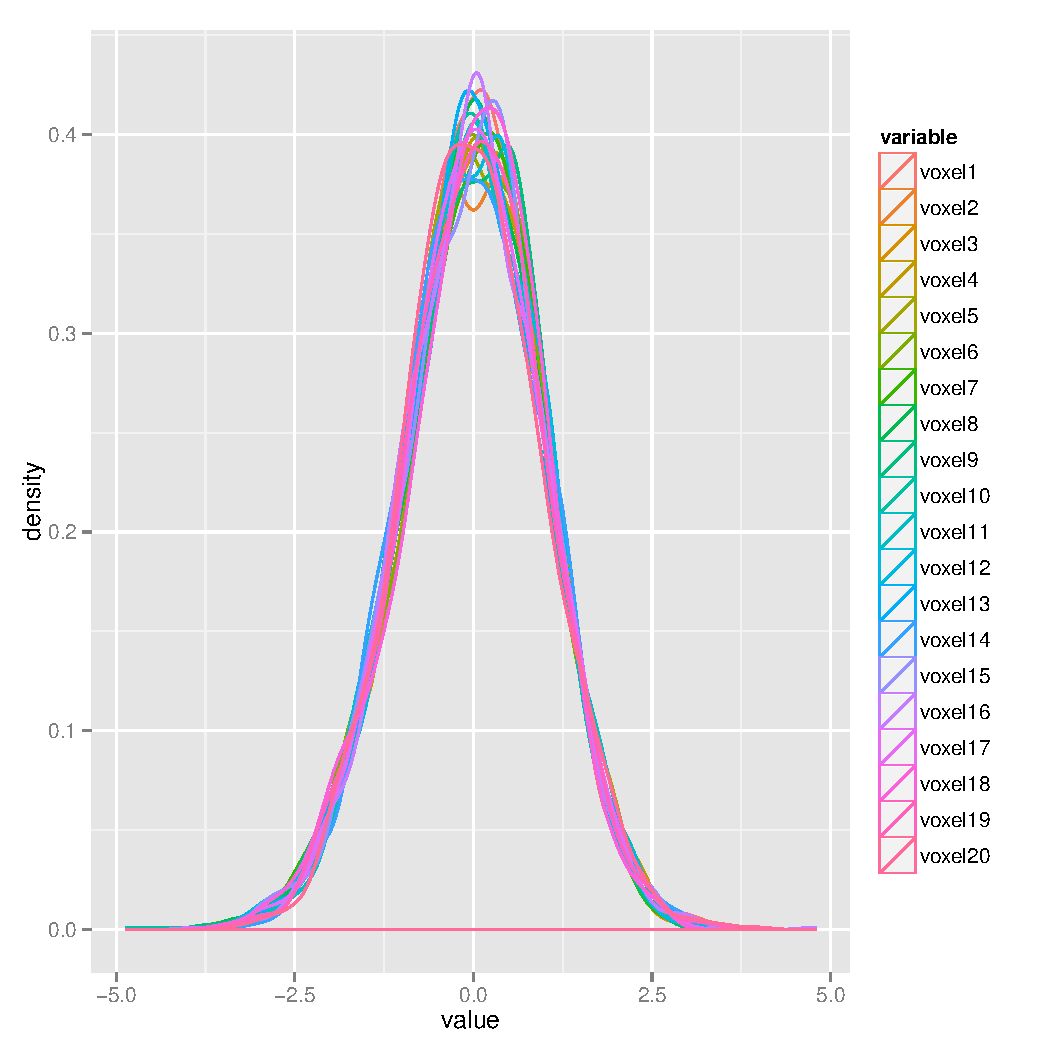
\includegraphics[width=\linewidth, height = 100pts]{response_density_EDA.pdf}
\endminipage\hfill
\minipage{0.33\textwidth}%
  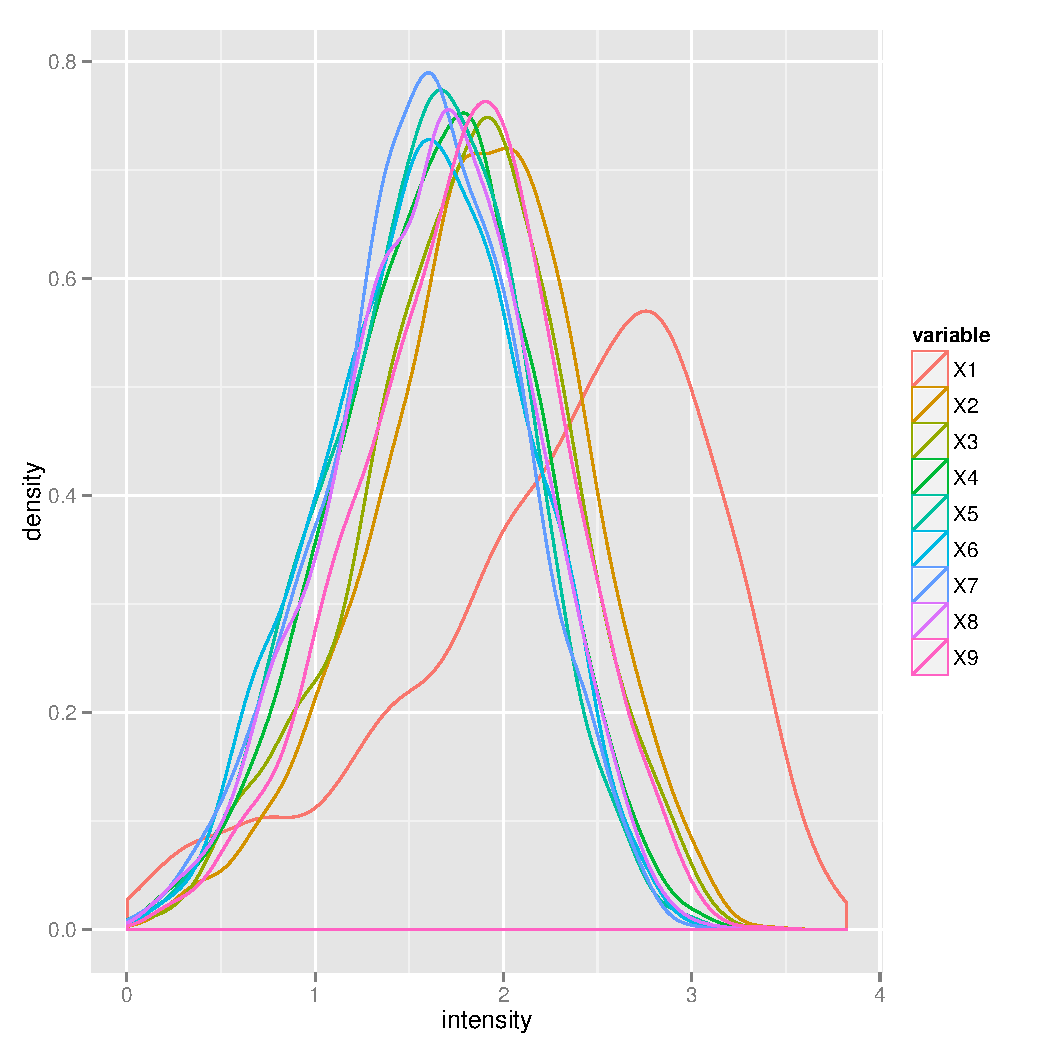
\includegraphics[width=\linewidth, height = 100pts]{intensity_density_EDA.pdf}
\endminipage
  \caption{}\
\end{figure}

The first figure graphs where the 20 voxels lie with respect to each other.  The voxels were coloured by splitting up one of the axis in half to give better depth perception.  We are aware that the topology of our visual field is preserved in the mapping of stimulus to V1.  We don't know how this mapping relates to the euclidean distance of the voxels, but it keeps us thinking about whether voxels that are further far apart are in charge of further parts of the visual field.  We will check this assumption in the interpretation part of the lab.  \\

The other two plots above give us an idea of the density of measurements, across voxels (middle figure) and for the first 10 features (leftmost figure).  The density of intensities across voxels is comparably distributed, and normal-like.  The density of coefficients is less so, we see there are some which remain 0.  This motivates our normalizing the feature dataset before performing analysis.  

\section{LASSO}

\subsection{Preprocessing}
Before doing LASSO, and any of the other models, we centered and scaled our feature data.  In the case of feature shrinkage in regression models, this ensures the penalty will effect all features equally.  Since each feature is a coefficient of the Gabor wavelets, they are not initially on a comparable scale, hence the need to scale by the standard deviation of each feature column.  

\subsection{Model Selection: CV, ES-CV, AIC, BIC, AICc}

LASSO provides a family of regression models parametrized by the penalty magnitude $\lambda$; the greater the $\lambda$ the more degrees of freedom we lose.  In our problem $p >> n$, so feature shrinkage is needed. Choosing the right value of lambda to minimize the prediction error, yet not overfit, and demonstrate stability, comprise our model selection criteria.  AIC, BIC and AICc don't provide theoretical guarantees for this high dimensional regime, but it is interesting that they do corroborate the choices of lambda by CV and ES-CV as seen by the graphs below.  We select the graphs for voxels 1, 5, 10, 15, 20, as they maximize the physical distance between voxels. 10 and 20 seem to be outliers, as the graphs of the rest of the voxels, not displayed in this lab, resemble that of voxel 1. Compared to other feature shrinkage models, LASSO has the added benefit of interpretability; the $L^1$ norm is "pointy" on the axis (given by the feature set) and thus sends feature to 0 with increasing $\lambda$.   We analyze the model performance of 100 models per voxel, parametrized by a grid of 100 possible lambda values.\\

The following plots of full of information.  Cross validation was performed on 80\% of the 1750 data points.  The remaining 20\% was left for testing.  We tried both 5 fold and 10 fold cross validation, reporting below the results for 10 fold cross validation as they provided more stable ESCV results, but ultimately the conclusions did not change.  We present three methods from choosing an optimal lambda from the cross validation folds, Lambda.min, Lambda.1se and ES-CV.  Lambda.min corresponds to  the $\lambda$ that minimizes cross validation error, and is displayed by the leftmost vertical line in the CV plots.  The right-most line corresponds to Lambda.1se, which is the largest lambda that we can get away with that is within 1 stander error from Lambda.min.  This choice of $\lambda$ channels the philosophy that we move in the direction of increasing regularization; all else being equal, we go for the simpler solution.   \\

The graphs are aligned so one can compare the lambda chosen by CV methods with the AIC, BIC and AICc plot.  Though the latter three estimators achieved minimums for the largest lambda in the domain of lambdas considered, there is an obvious point at which their derivative decreases dramatically, to a almost flat slope.  This was the point that almost always corresponded to the lambdas chosen by CV methods within a small degree of error, hence providing nice support for the choices made by CV methods.  Finally, we can read of the degrees of freedom of the LASSO model for each voxel on the top of the x-axis, which consistently chose around 90 parameters at Lambda.min. Voxel 10, 16 and 20 were outliers.  

\begin{figure}[H]
\minipage{0.45\textwidth}
  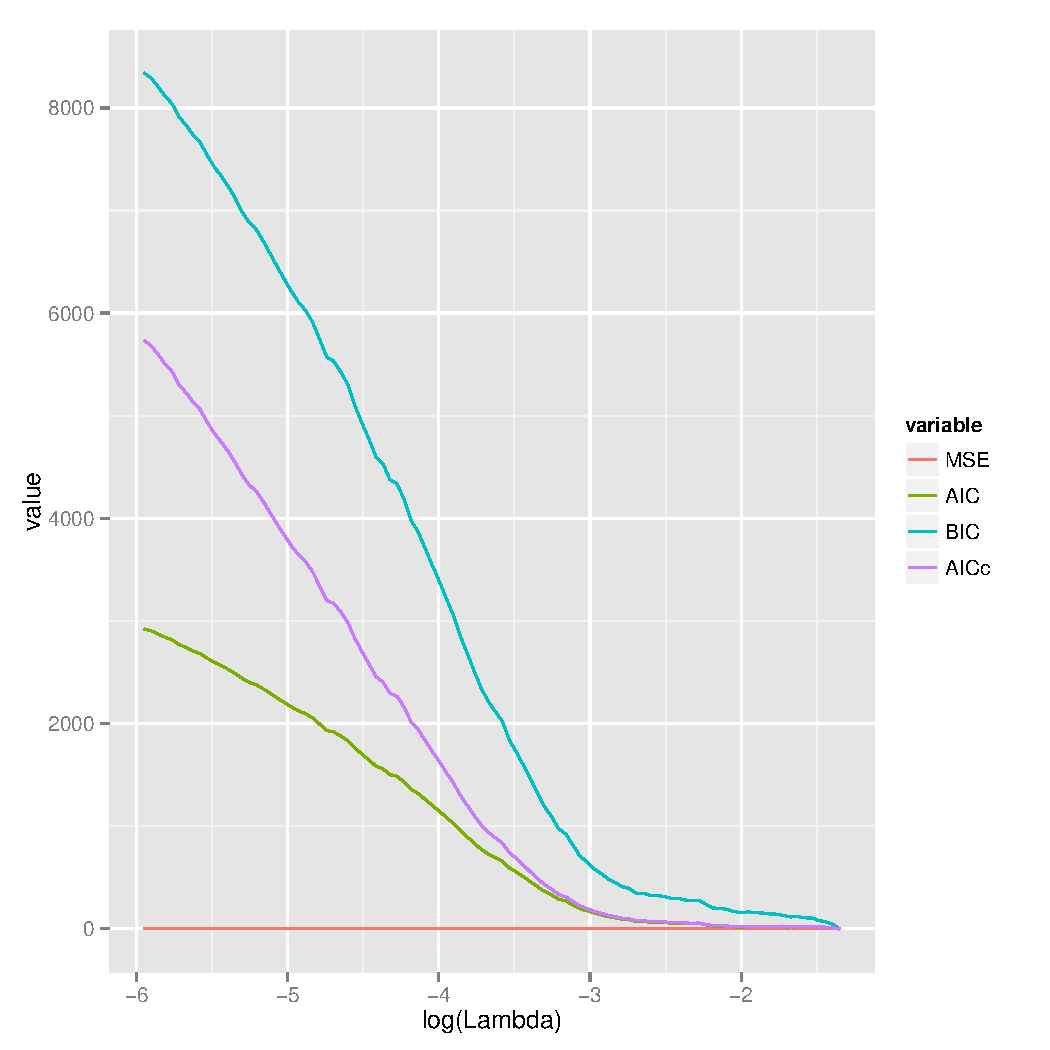
\includegraphics[width=\linewidth]{Voxel_1_AIC.pdf}
  \caption{Voxel 1}
\endminipage\hfill
\vspace{-5mm}
\minipage{0.45\textwidth}
  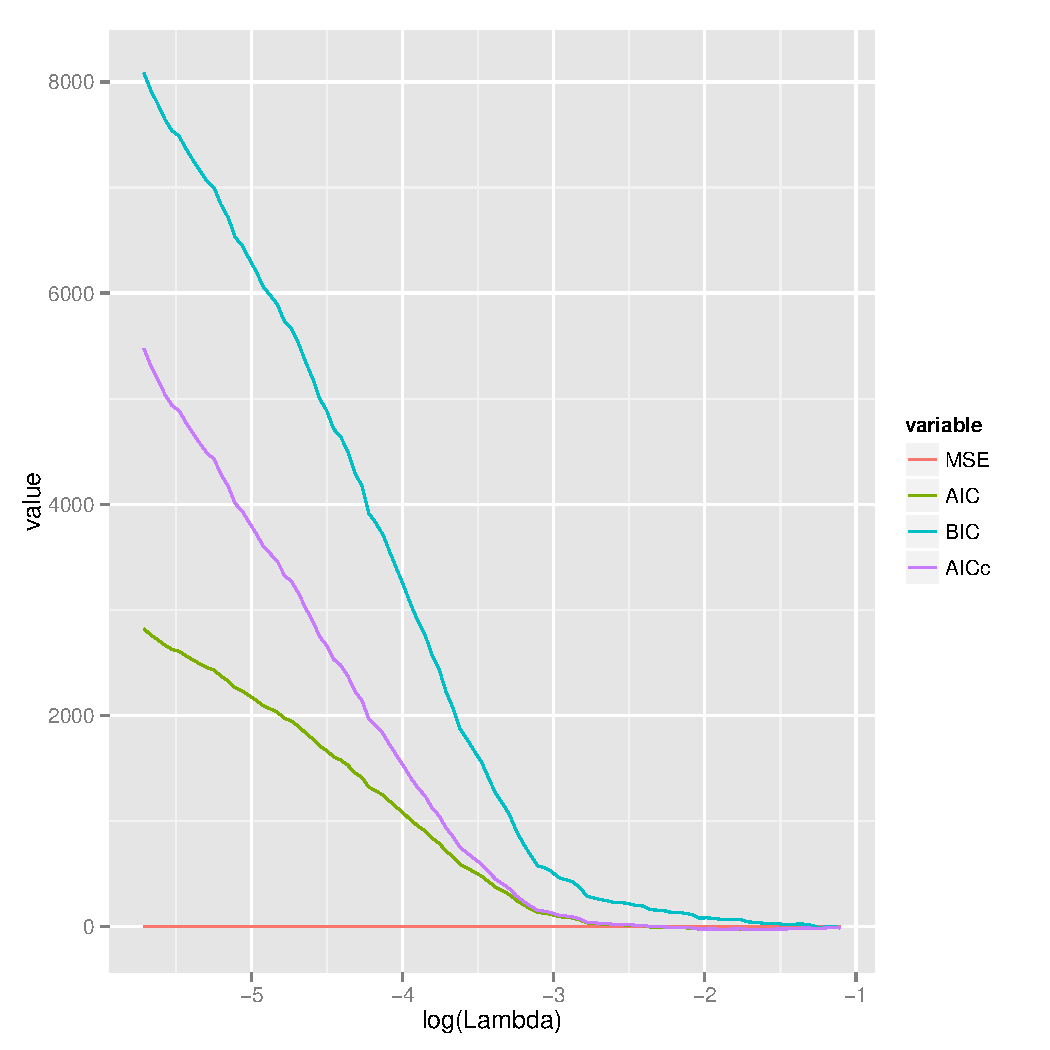
\includegraphics[width=\linewidth]{Voxel_5_AIC.pdf}
  \caption{Voxel 5}
\endminipage
\caption{AIC, BIC, AICc}

\end{figure}
\vspace{-20mm}

\begin{figure}[H]
\minipage{0.45\textwidth}
  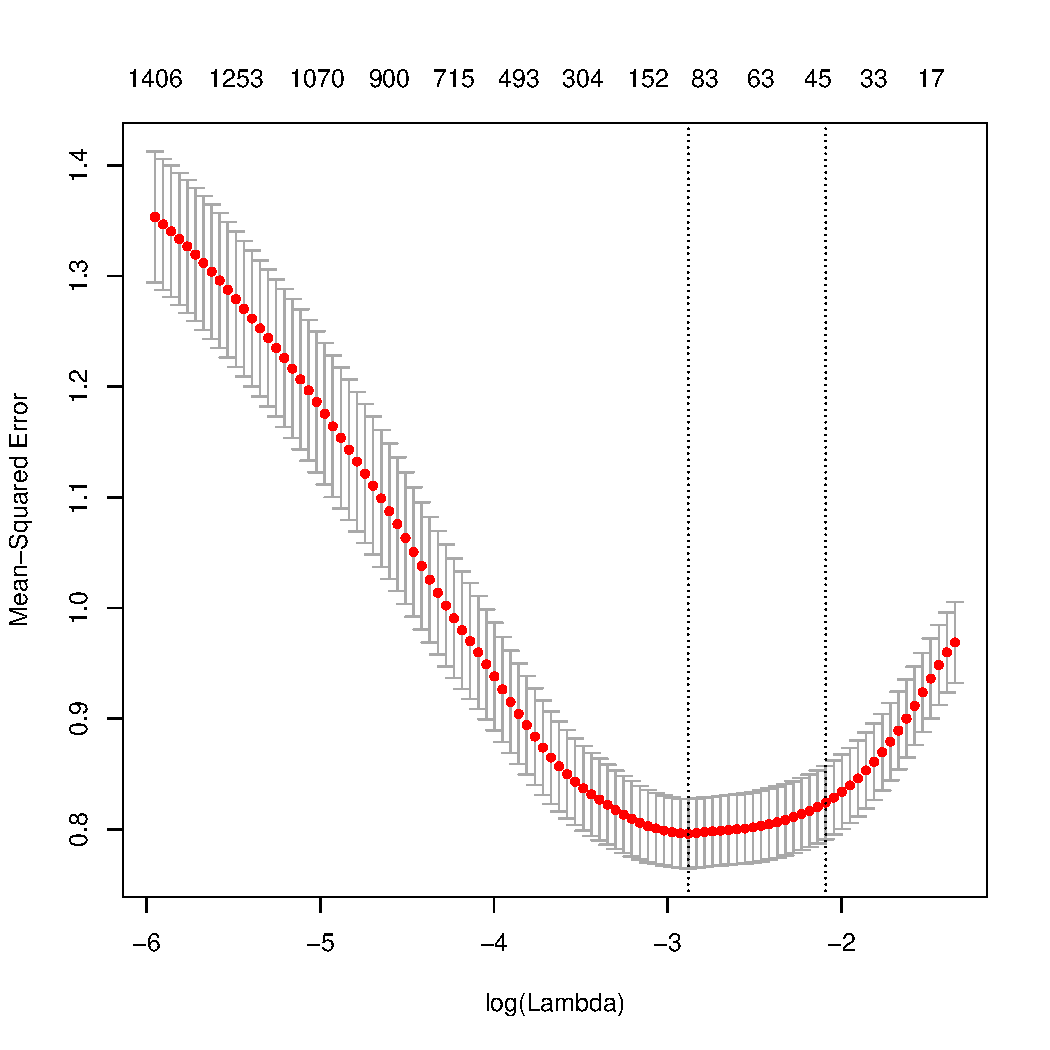
\includegraphics[width=\linewidth]{cv_lasso1.pdf}
  \caption{Voxel 1}
\endminipage\hfill
\vspace{-5mm}
\minipage{0.45\textwidth}
  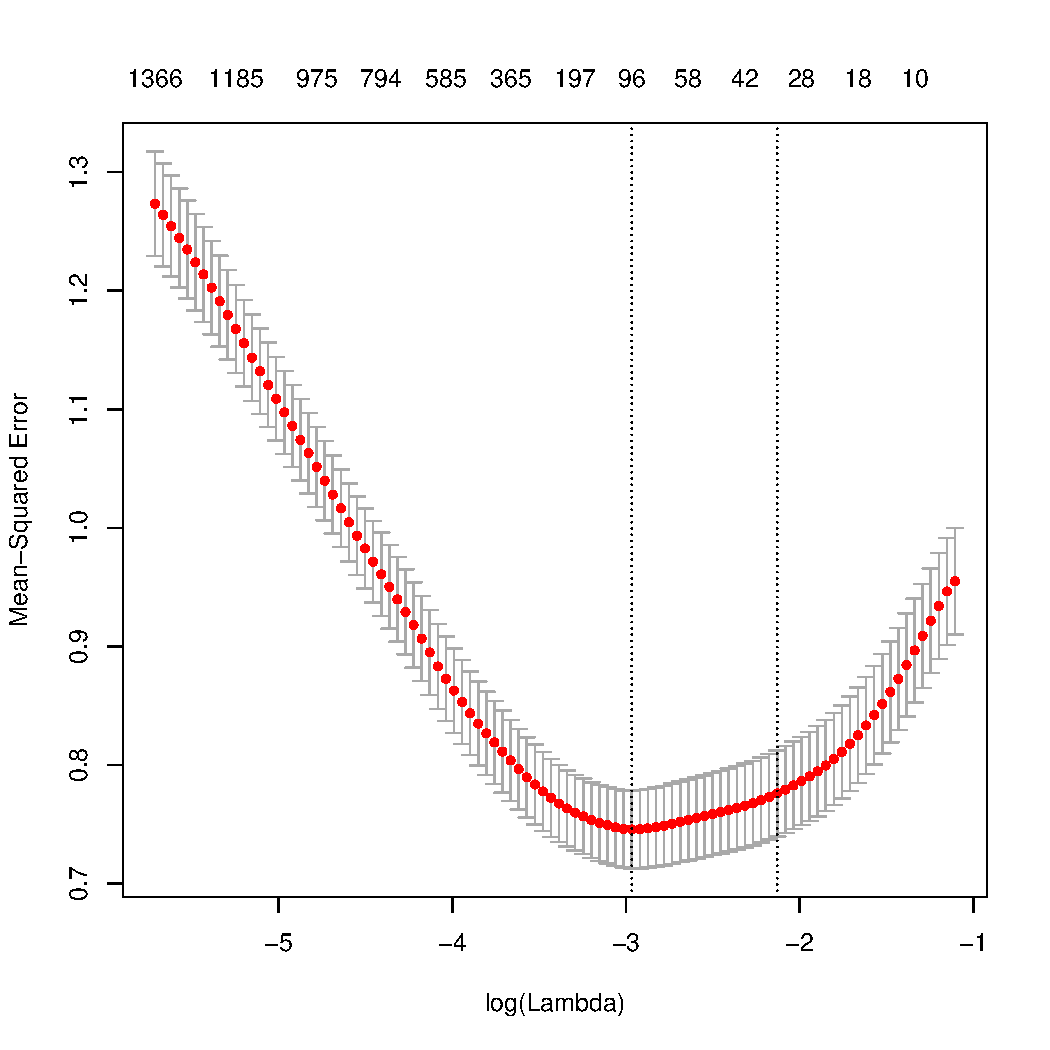
\includegraphics[width=\linewidth]{cv_lasso5.pdf}
  \caption{Voxel 5}
\endminipage
\caption{Cross Validation Selection of Lambda}
\end{figure}
\vspace{-20mm}

\begin{figure}[H]
\minipage{0.45\textwidth}
  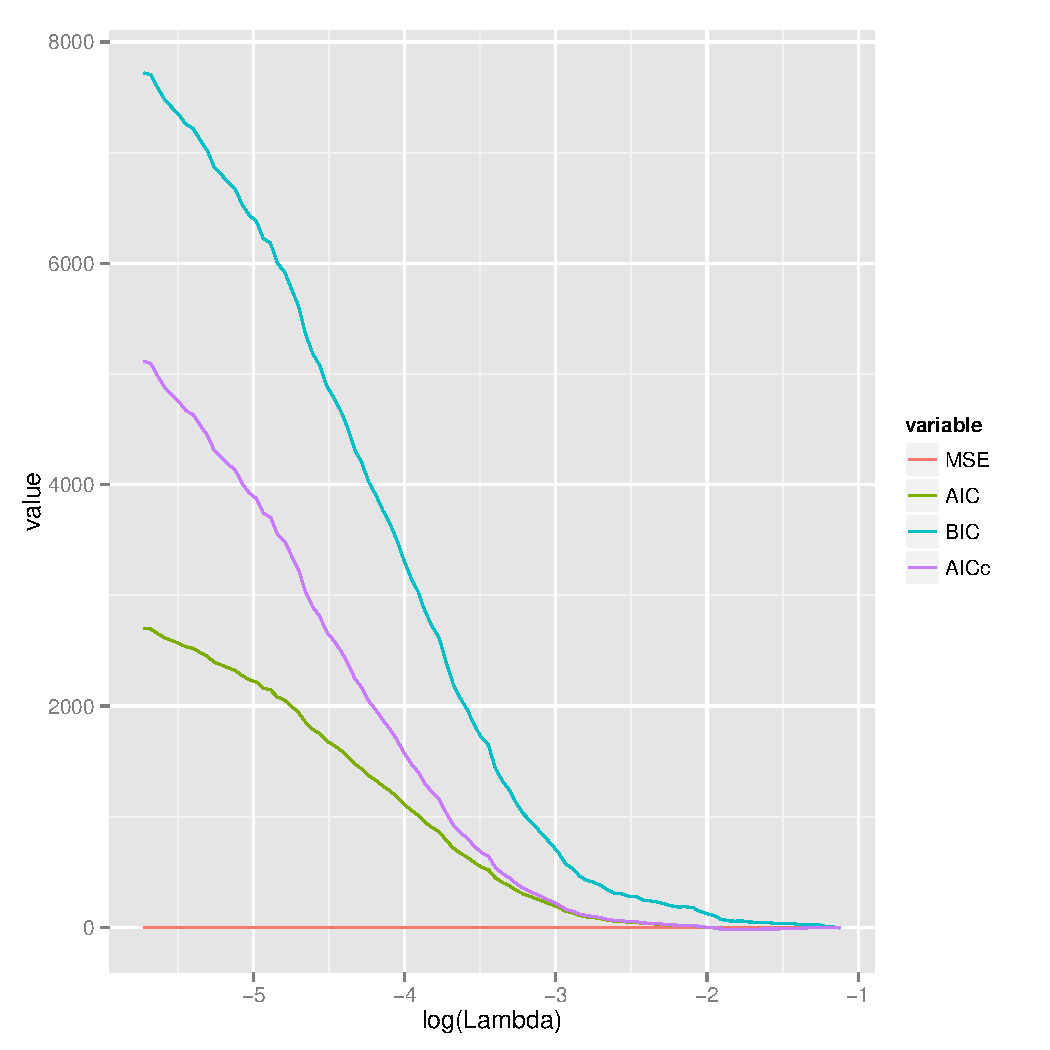
\includegraphics[width=\linewidth]{Voxel_15_AIC.pdf}
  \caption{Voxel 15}
\endminipage\hfill
\vspace{-5mm}
\minipage{0.45\textwidth}
  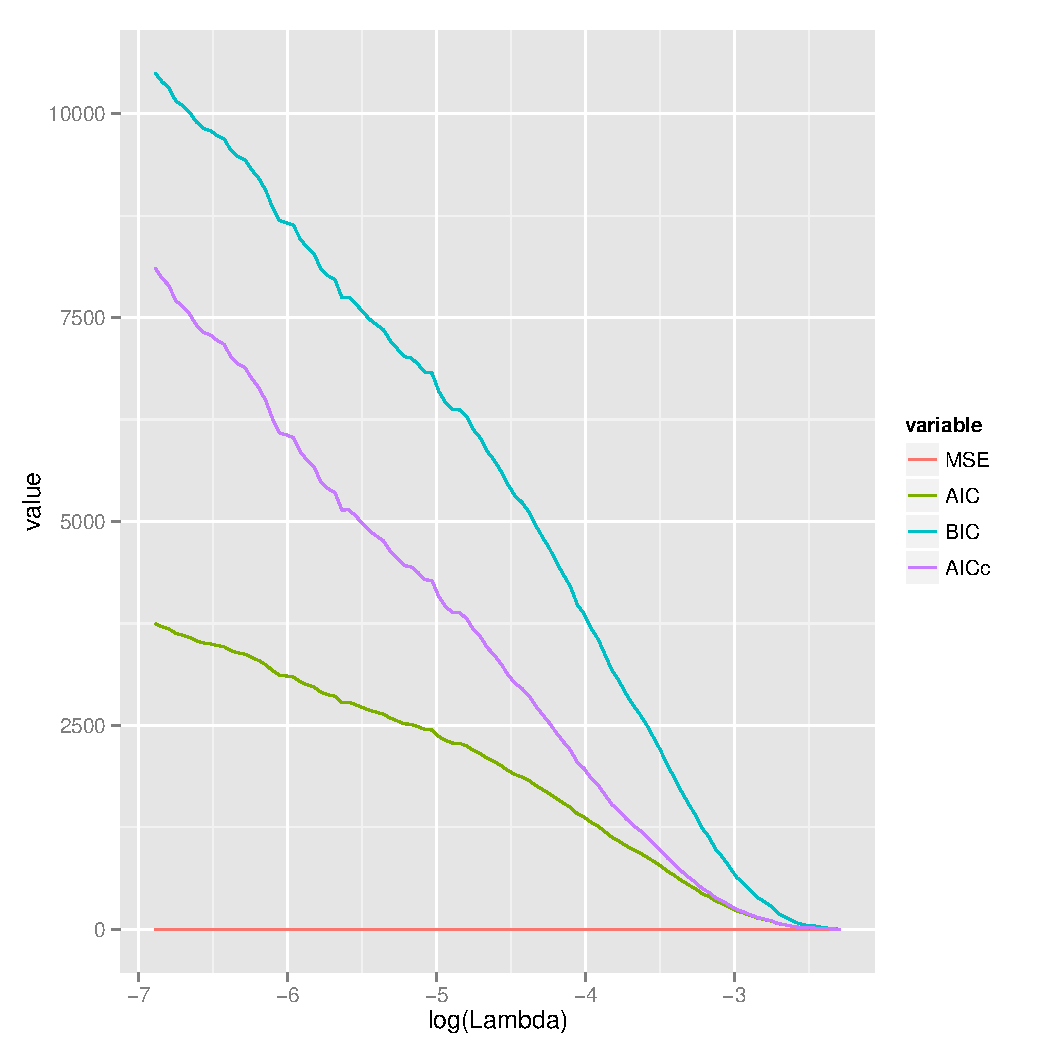
\includegraphics[width=\linewidth]{Voxel_20_AIC.pdf}
  \caption{Voxel 20}
\endminipage
\caption{AIC BIC AICc}
\end{figure}
\vspace{-20mm}

\begin{figure}[H]
\minipage{0.45\textwidth}
  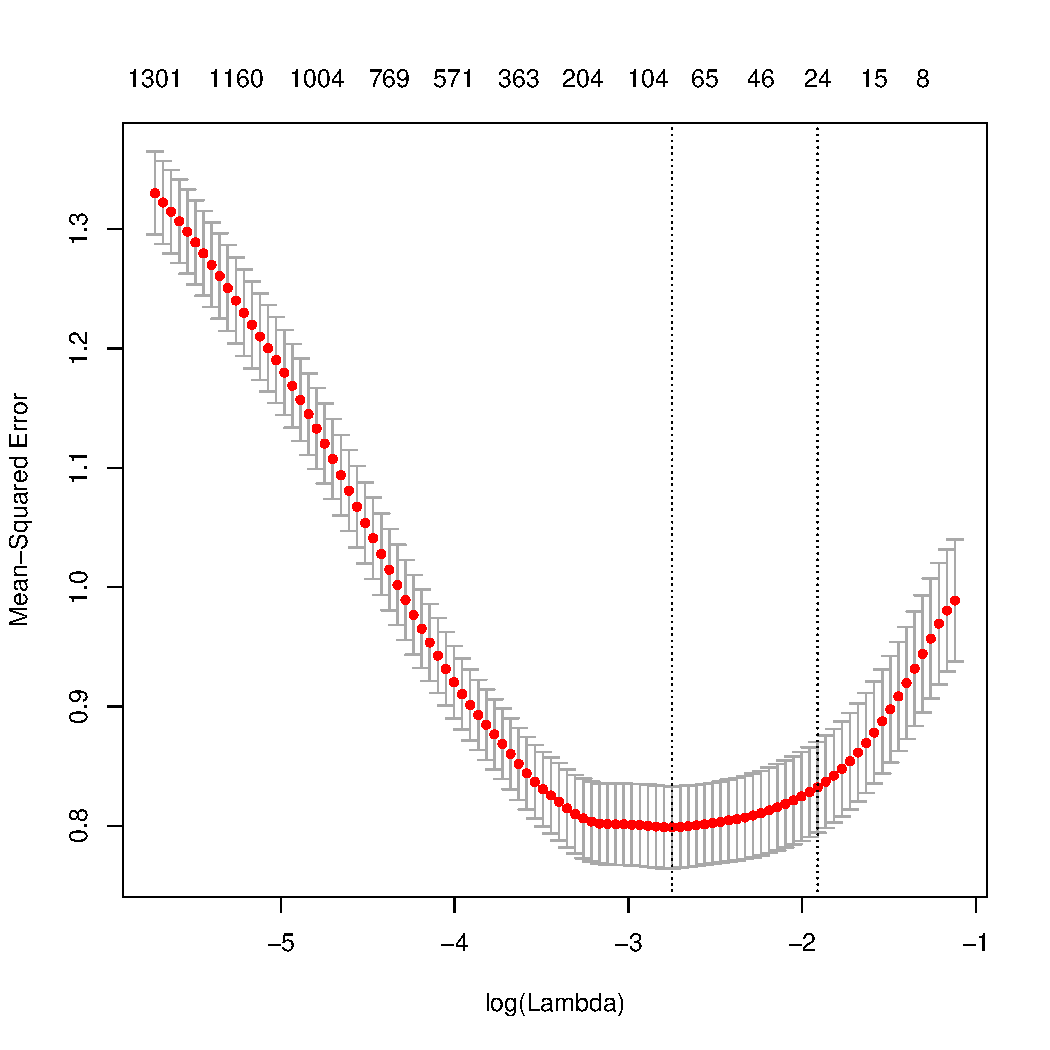
\includegraphics[width=\linewidth]{cv_lasso15.pdf}
  \caption{Voxel 15}
\endminipage\hfill
\vspace{-5mm}
\minipage{0.45\textwidth}
  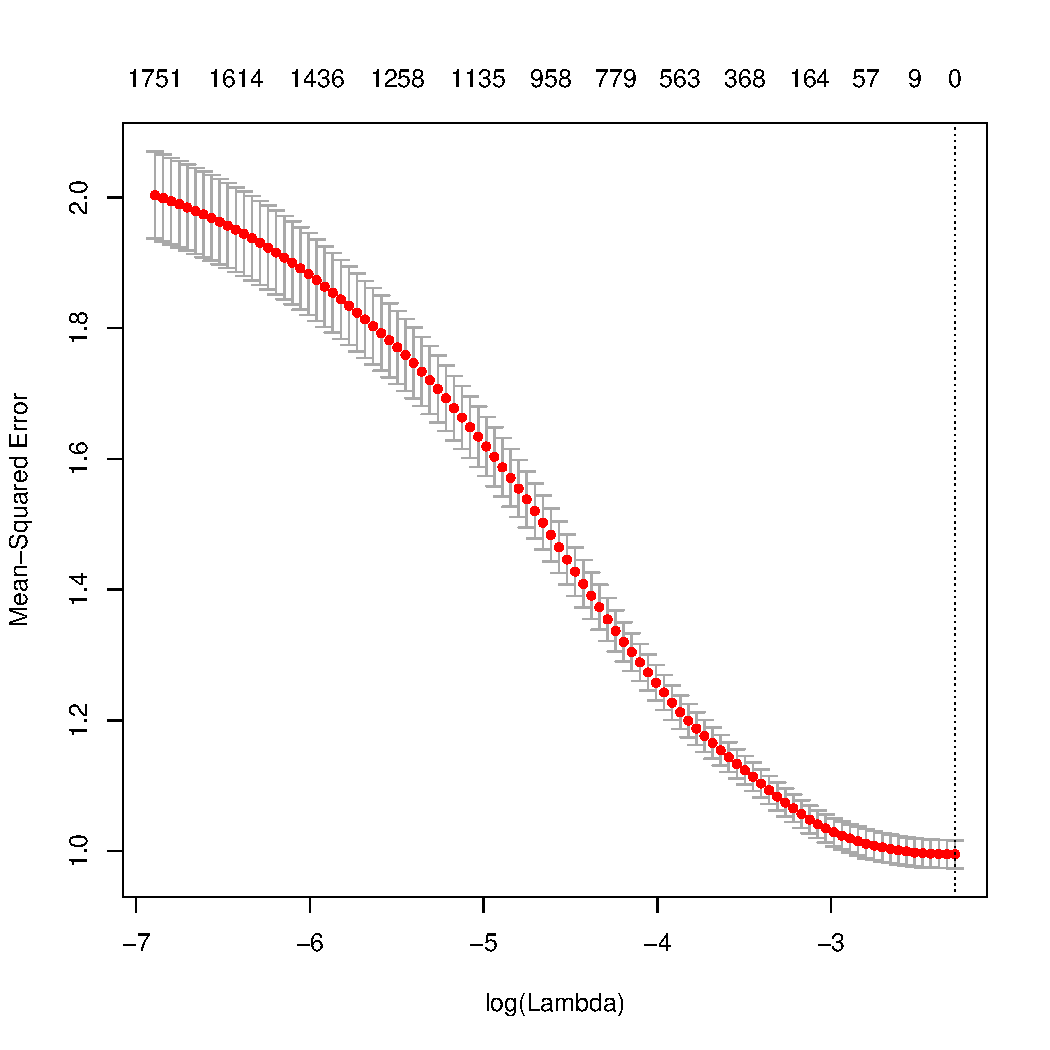
\includegraphics[width=\linewidth]{cv_lasso20.pdf}
  \caption{Voxel 20}
\endminipage
\caption{Cross Validation Selection of Lambda}
\end{figure}
\vspace{-20mm}


\begin{figure}[H]
\minipage{0.45\textwidth}
  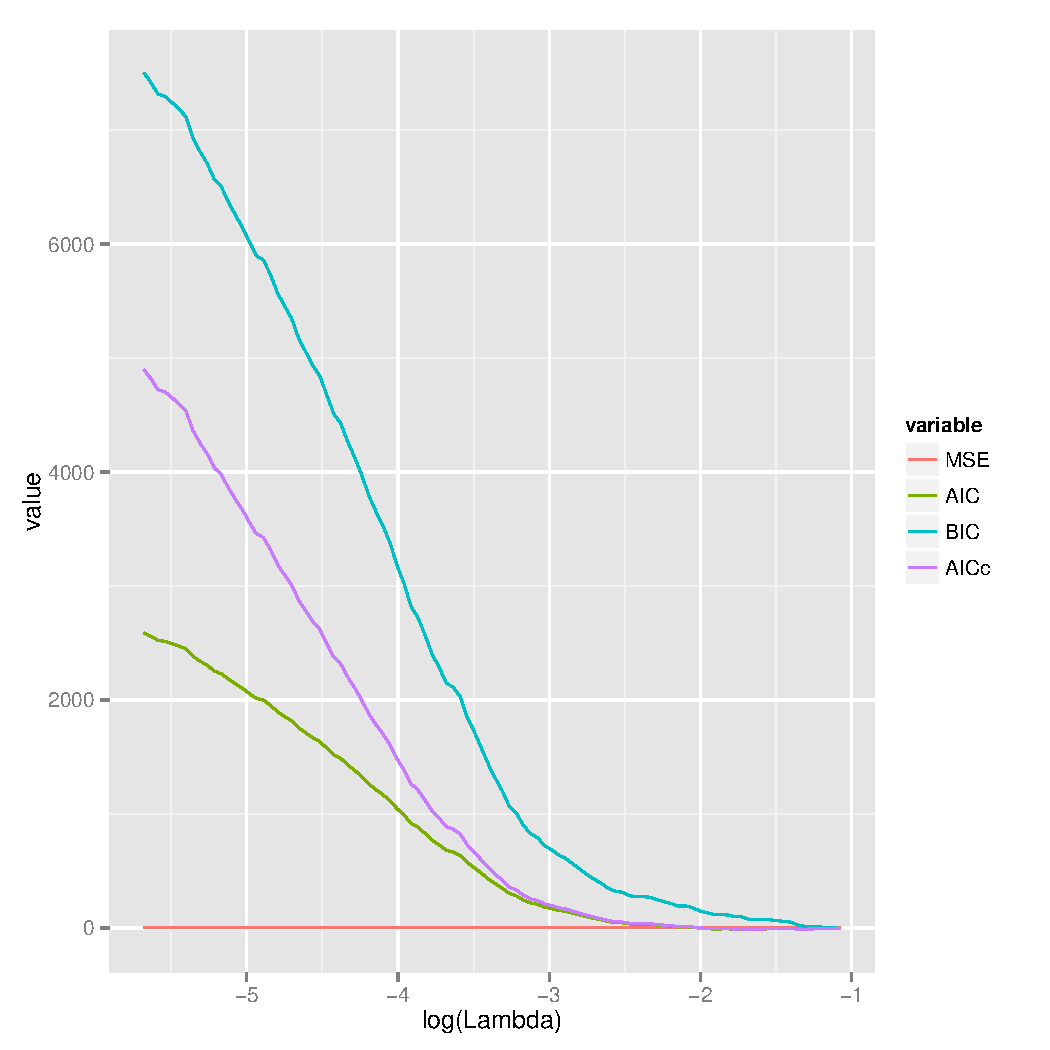
\includegraphics[width=\linewidth]{Voxel_2_AIC.pdf}
  \caption{Voxel 16}
\endminipage\hfill
\vspace{-5mm}
\minipage{0.45\textwidth}
  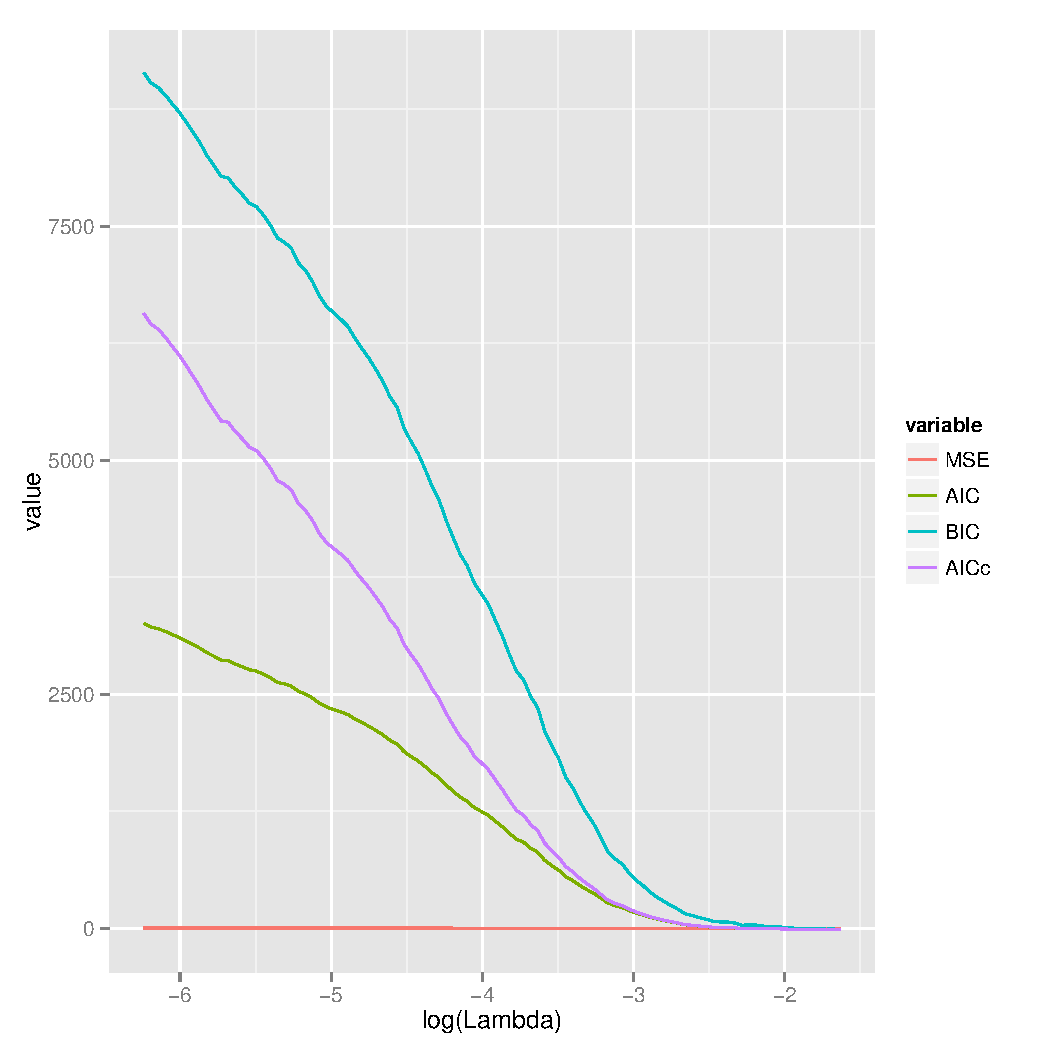
\includegraphics[width=\linewidth]{Voxel_10_AIC.pdf}
  \caption{Voxel 10}
\endminipage
\caption{AIC, BIC, AICc}
\end{figure}
\vspace{-20mm}


\begin{figure}[H]
\minipage{0.45\textwidth}
  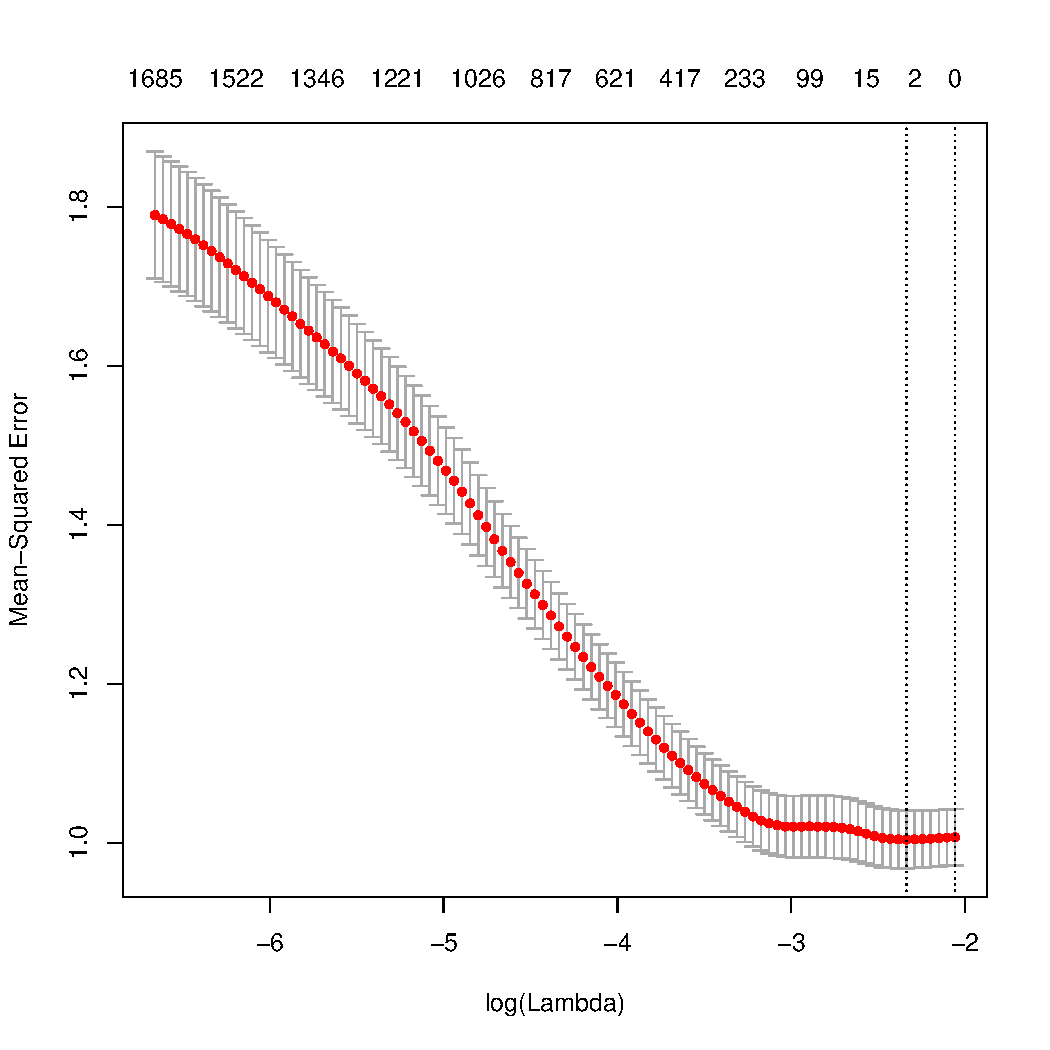
\includegraphics[width=\linewidth]{cv_lasso16.pdf}
  \caption{Voxel 16}
\endminipage\hfill
\vspace{-5mm}
\minipage{0.45\textwidth}
  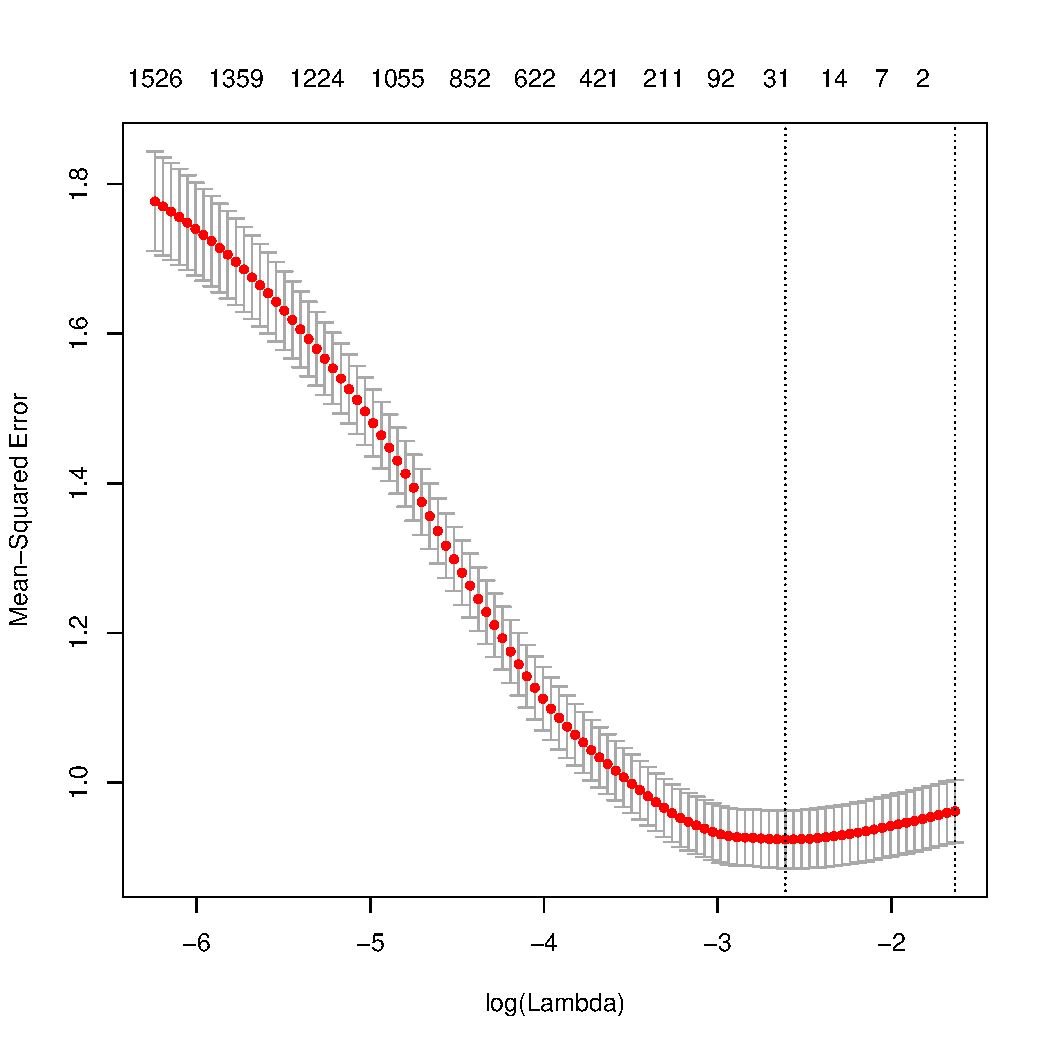
\includegraphics[width=\linewidth]{cv_lasso10.pdf}
  \caption{Voxel 10}
\endminipage
\caption{Cross Validation Selection of Lambda}
\end{figure}
\vspace{-10mm}

ESCV plots: 

\begin{figure}[H]
\minipage{0.58\textwidth}
  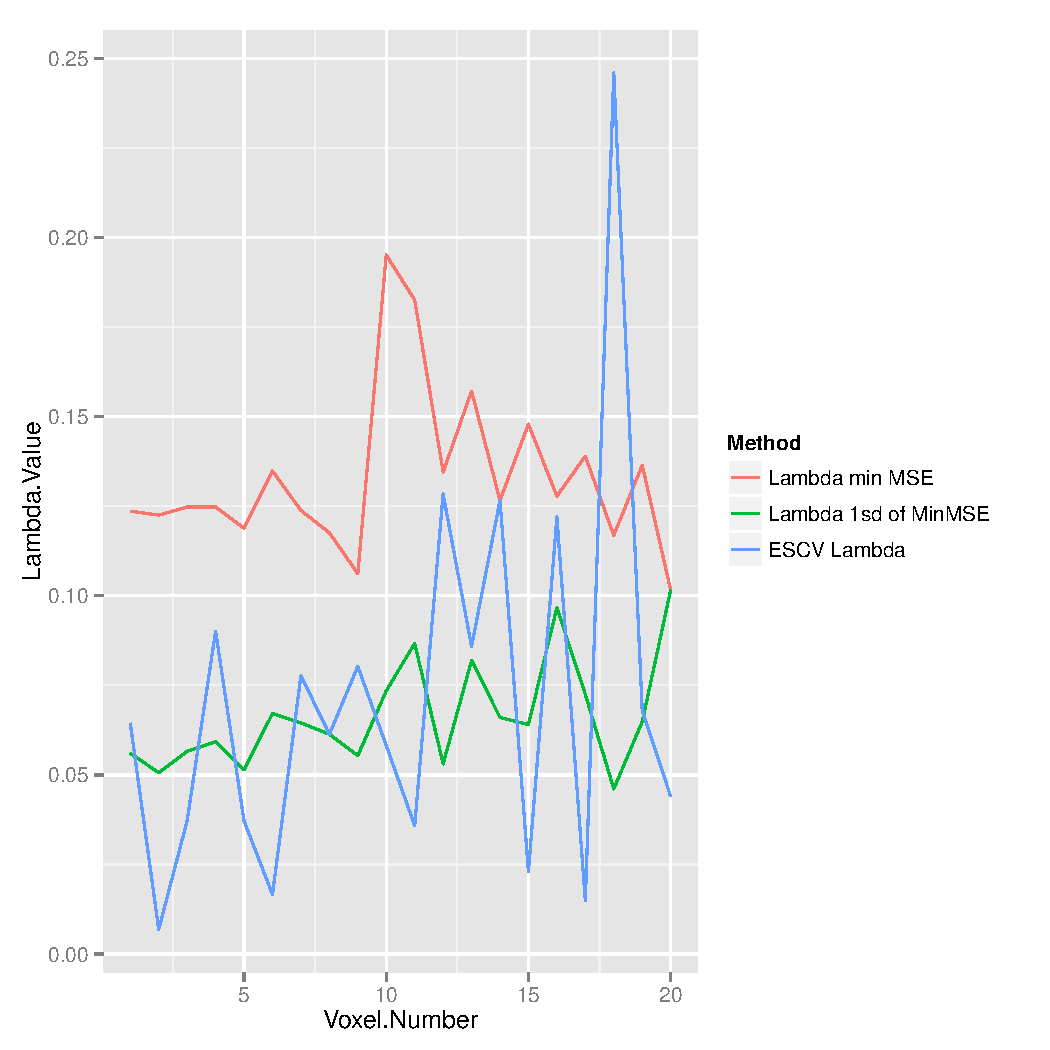
\includegraphics[width=\linewidth, height=200pts]{lambda_value.pdf}
  \caption{Lambda selection using CV, CVsd and ESCV}
\endminipage\hfill
\vspace{-5mm}
\minipage{0.32\textwidth}
  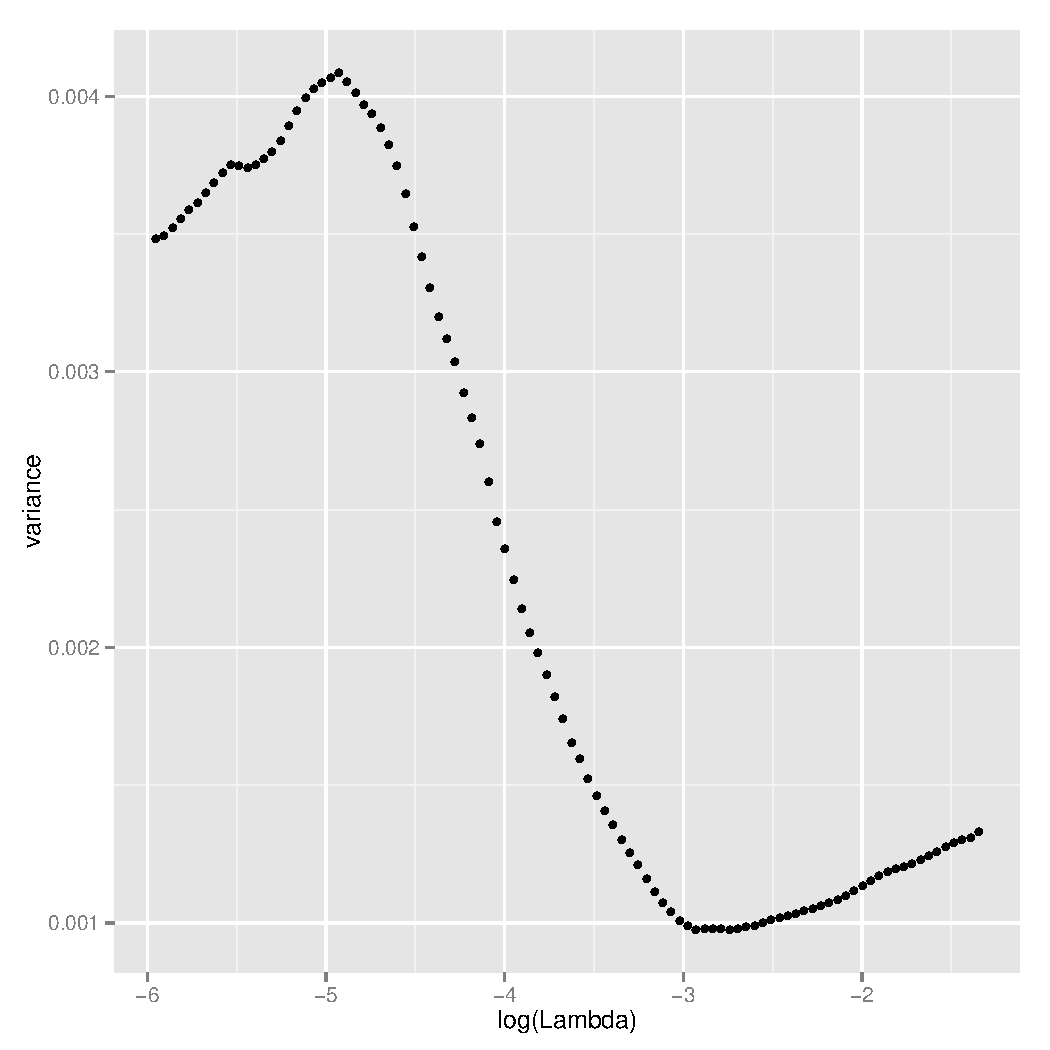
\includegraphics[width=\linewidth]{Voxel_1_ESCV.pdf}
  \caption{ESCV Voxel 1}
\endminipage
\end{figure}

The figure on our top left is a plot of lambda values chosen across voxels and compares them across the three methods using cross validation to choose $\lambda$.  By definition Lambda.1se will always be greater than Lambda.min.  It is interesting that ES-CV seems to fall more or less in the middle (my implementation was slightly flawed, as by definition, I was supposed to choose an argmin that was greater than Lambda.min, thus, we should interpret the ESCV below Lambda.min as lying on Lambda.min).  Lambda.min and Lambda.1se choose fairly consistent penalty terms across voxels, which motivates one to try using the same lambda, chosen optimally by implementing LASSO via multi response option in glment.  Unfortunately, as we will discover in the later section, it did not provide a satisfactory correlation plot (later section) as our lambdas chosen by Lambda.min or Lambda.1se.  This may very well be due to voxel 10 and 20 being outliers (having barely any variance and thus outputting a prediction of constant response to all pictures).  

\begin{figure}[H]
\minipage{0.68\textwidth}
  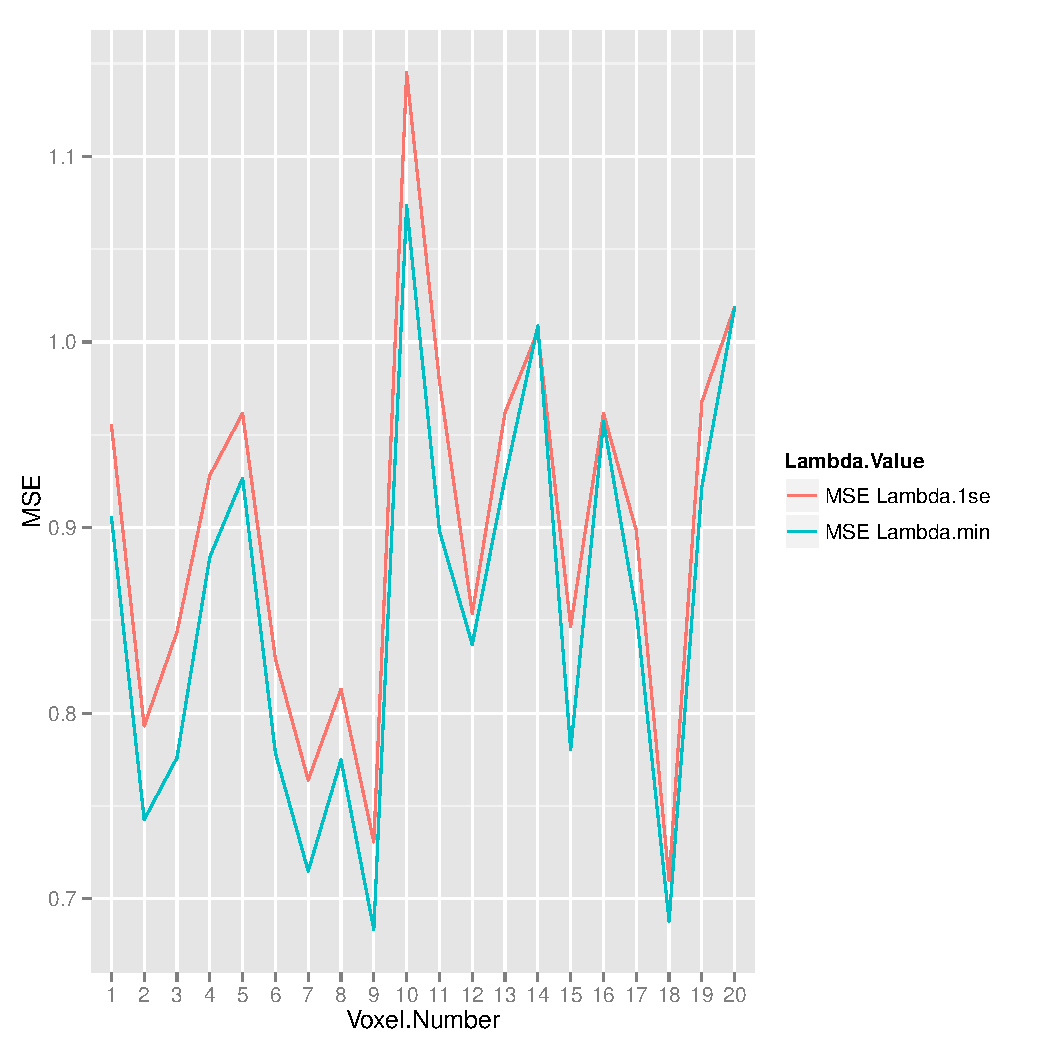
\includegraphics[width=\linewidth, height=250pts]{MSE_lambda_plot.pdf}
  \caption{Voxel 1}
\endminipage\hfill
\minipage{0.3\textwidth}
To our left we see a plot of the mean squared error (MSE) of the predicted response vector given the $\lambda$ selected by ESCV, lambda.min and Lambda.1se.  It is worth noting on average Lambda.min required 90 parameters whereas Lambda.1se required half as many, making it a more ideal choice for a more interpretable model.  The MSE is taken from the 20\% test set, that was not part of the original training set of the cross validated models.  

\endminipage
\end{figure}


\section{Correlation between voxels} Below we give the correlation plots between voxels for three of our LASSO models:  Lambda.min, Lambda.1se and Lambda.min chosen by multi response Gaussian LASSO.  We also plot the original correlation plot between voxels for comparison.  In the correlation plots corresponding to the three prediction models, voxels across the top represent the predicted responses, and those on the vertical are the actual.  We satisfyingly see that Lambda.min and Lambda.1se do an excellent job at recovering the gestalt of correlation information of the original voxels, though they are greatly weakened (for instance, between actual and predicted, we have a range of out 0.35-0.55 correlation).  Precise numbers can be found in the table of correlations for the LASSO using Lambda.min is provided in Appendix I.  It is worth noting that voxel 10, 16 and 20 already appear to be outliers according to the original correlation plot.  The model provided by the multi response gaussian did not fare as well, and we are not surprised since there are 3/20 outliers, this would affect a model that chooses the same $\lambda$ for all voxels. 
   \\  
\begin{figure}[H]
\minipage{0.45\textwidth}
  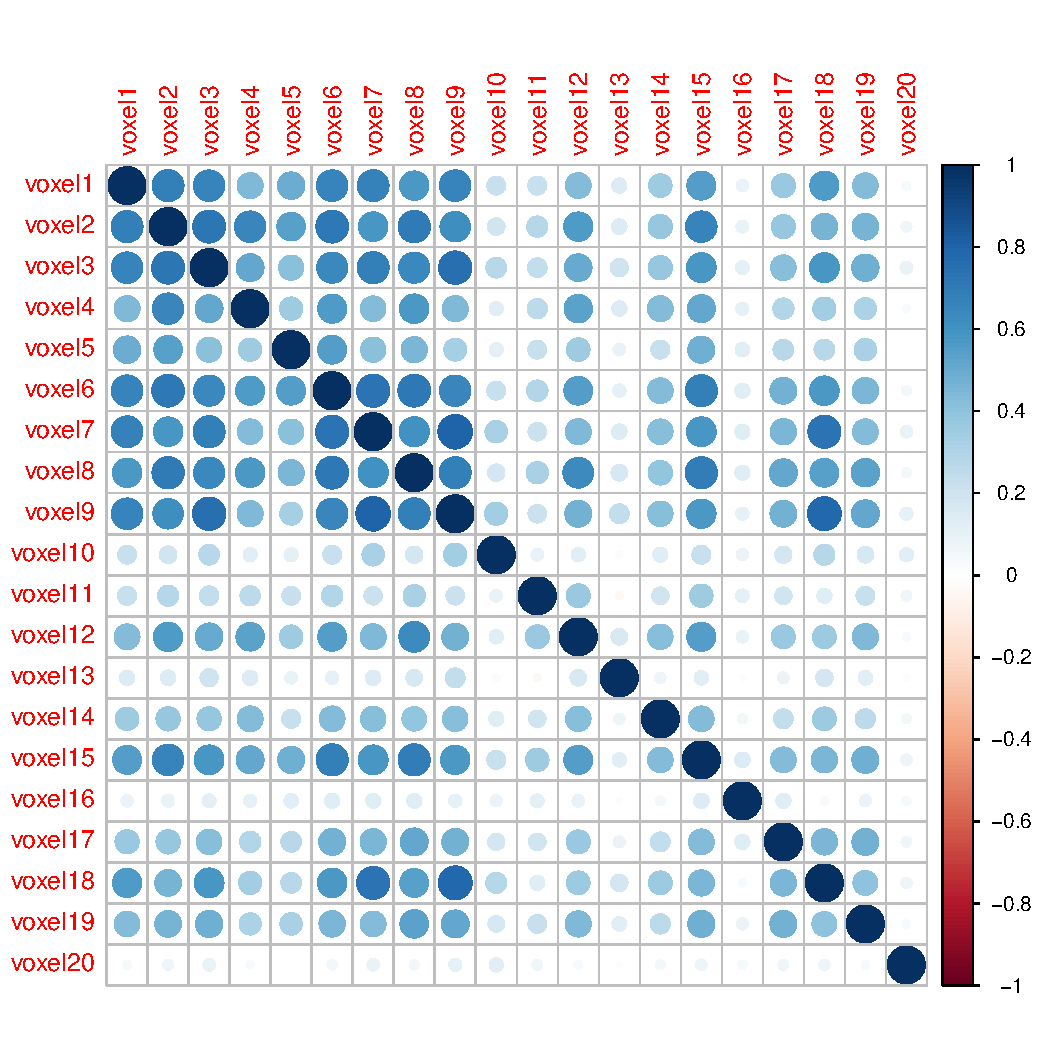
\includegraphics[width=\linewidth]{corrplot_actual.pdf}
  \caption{Original correlation}
\endminipage\hfill
\vspace{-5mm}
\minipage{0.45\textwidth}
  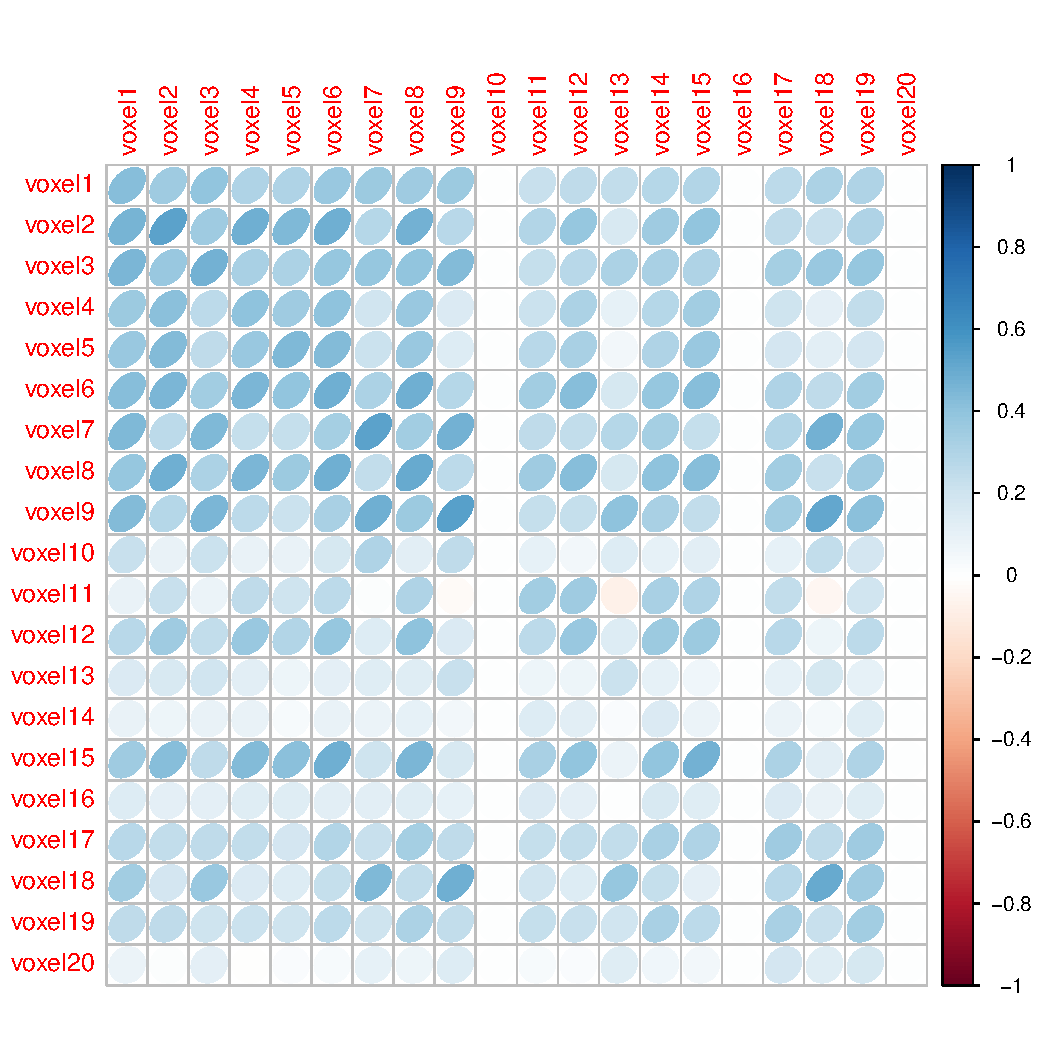
\includegraphics[width=\linewidth]{corrplot.pdf}
  \caption{Correlation for LASSO using Lambda.min}
\endminipage

\end{figure}

\vspace{-5mm}
\begin{figure}[H]
\minipage{0.45\textwidth}
  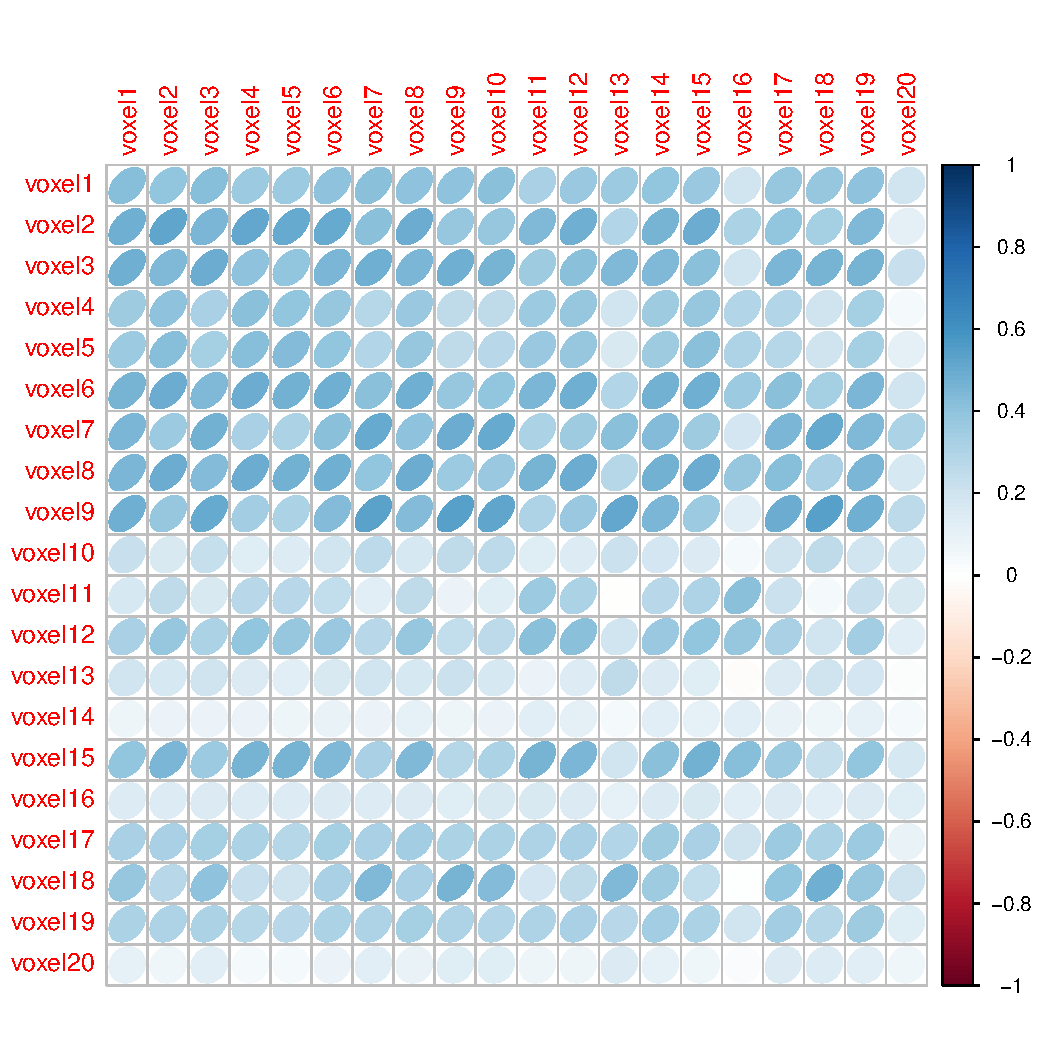
\includegraphics[width=\linewidth]{corrplot_mg.pdf}
    \caption{Correlation for Multigaussian LASSO Lambda.min}
\endminipage\hfill
\vspace{-5mm}
\minipage{0.45\textwidth}
  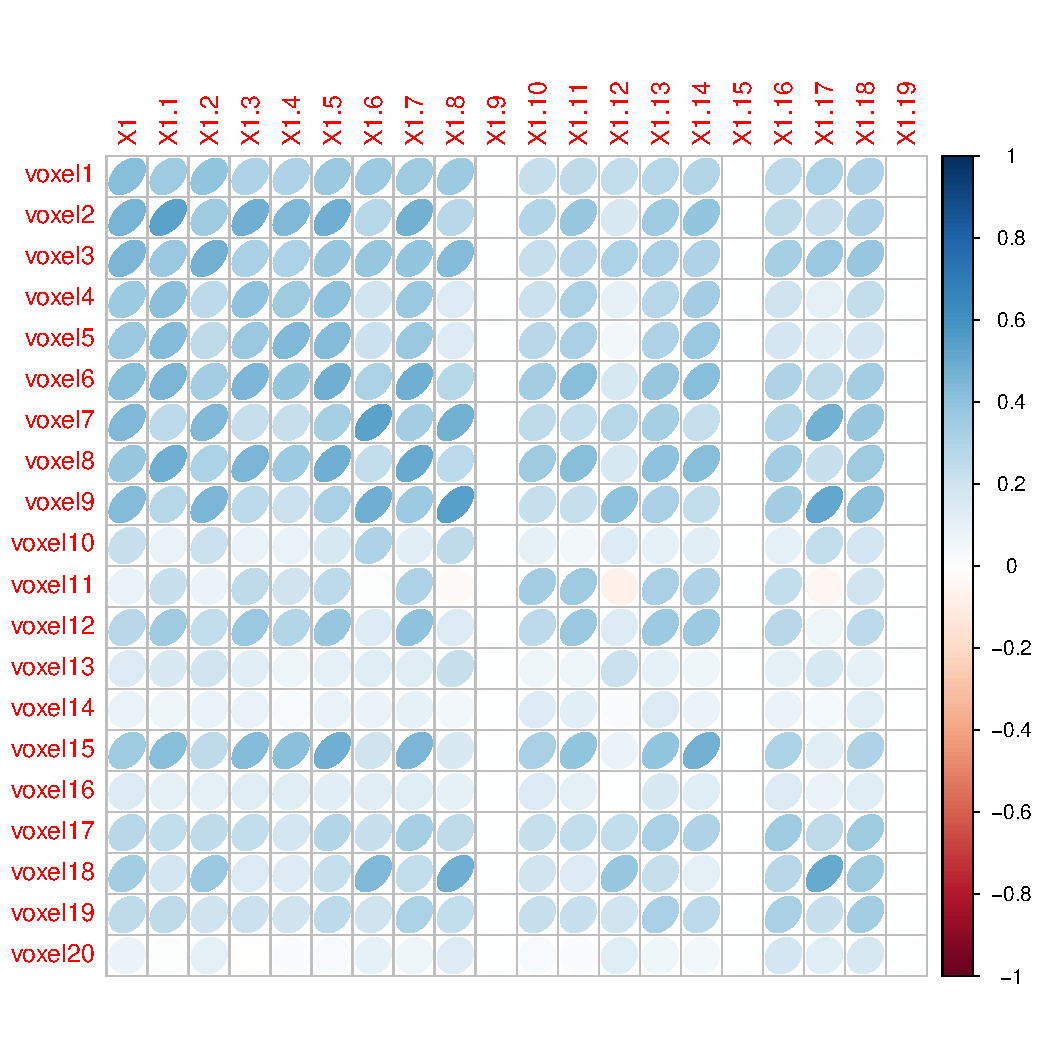
\includegraphics[width=\linewidth]{corrplot_1se.pdf}
    \caption{Correlation for LASSO Lambda.1se}
\endminipage


\end{figure}

\section{Ridge, mixture Ridge-Lasso, Random Forest}
Below we find the mean squared error (MSE) plotted against different choices of $\lambda$ for Ridge regression and a mixture of Ridge regression and LASSO. They are results for voxel 1. Though Ridge provided the the lowest MSE, it was the least interpretable model since it was not possible to pick out individual features in the reduced feature set (the degrees of freedom are reduced in Ridge, contrary to what is being plotted on the top of the x-axis, but it can only be measured by the trace of the penalized projection matrix).  The mixture model performed as well as LASSO, but owing on the simplicity of LASSO coefficient selection, we continued with the LASSO model.  Random Forest was also implemented, and with just 30 trees, it was able to achieve very low out of bag error.  It's performance on the test set with just 30 trees was comparable to LASSO (about 0.9), but once we increased our forest to 100 trees, we were able to reduce MSE to a little over 0.7.  There was not more improvement when using more than 100 trees were.  The reason why we did not continue with the random forest model in creating our predictor is because it is not interpretable at all, and so does not inform the original scientific question at hand.  

\begin{figure}[H]
\minipage{0.45\textwidth}
  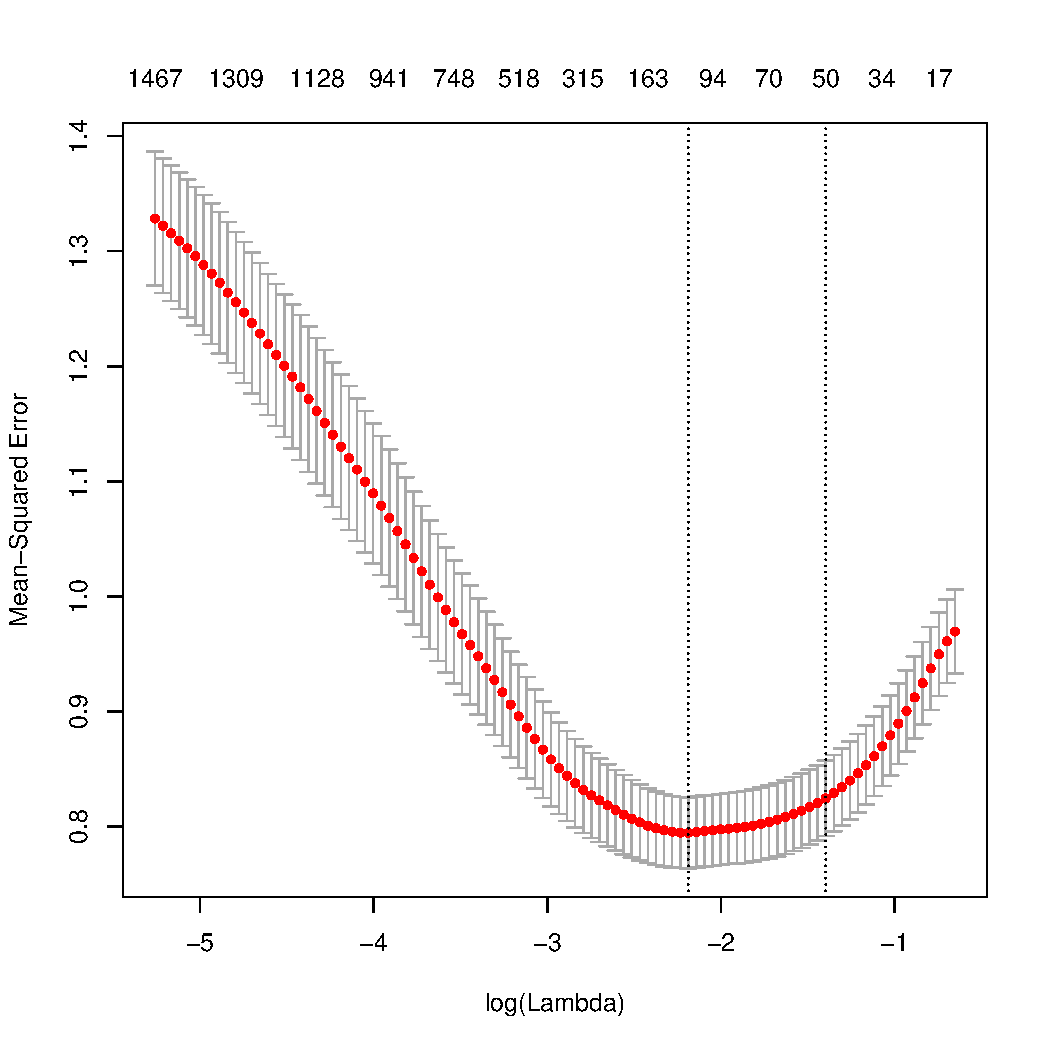
\includegraphics[width=\linewidth]{cv_lasso1_half.pdf}
  \caption{Mixture Ridge Lasso}
\endminipage\hfill
\vspace{-5mm}
\minipage{0.45\textwidth}
  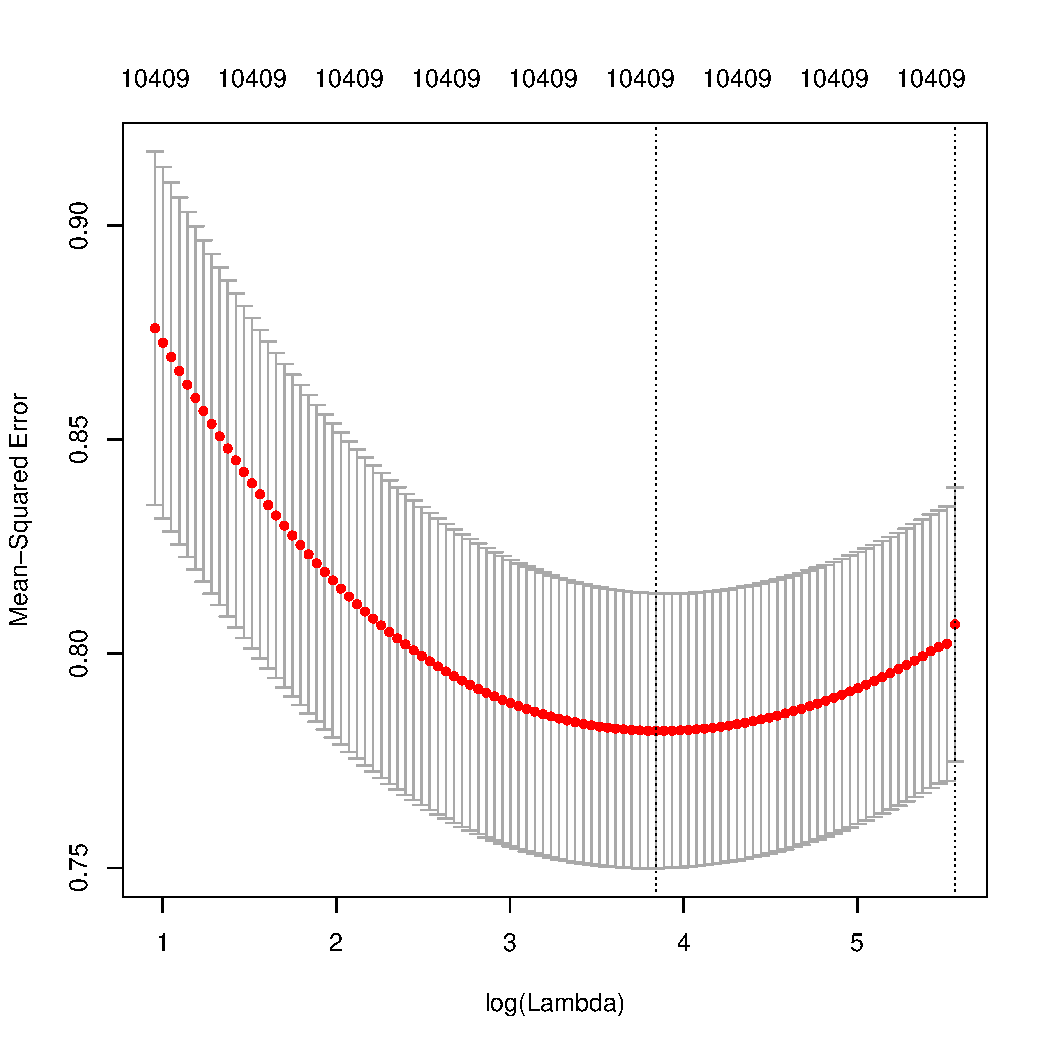
\includegraphics[width=\linewidth]{cv_ridge1.pdf}
\caption{Ridge}
\endminipage
  \caption{Lambda selection for Ridge and Ridge/Lasso Mixture}
\end{figure}

\section{Stability}

Two parallel analysis of the above tasks were actually conducted, one on a  50/50 split and 80/20 split of the original 1750 data points into training and testing set respectively.  Since the $n$ data points have no relations beyond being natural pictures, we randomly chose the training and test sets, sampling with replacement to get a bootstrapped population. This was justified as voxel responses and feature variables were clearly bounded.  Random Forest did well for 80/20, but not so well for 50/50, whereas the other regression methods performed similarly for both splits.  In particular, degrees of freedom and MSE error for the optimal $\lambda$s (chosen in the three ways) were robust with the two different splits of training and test.  Hence we choose to examine the regression models in more detail.  


\section{Feature Interpretation}

We tried studying the parameters given by the model by looking at the Gabor basis elements that voxel 1 and voxel 10's top 10 most important coefficients corresponded to.  We ranked importance based on the magnitude of the coefficients, since all features are on the same scale due to initial  centering and scaling.  A couple of interesting things were discovered (plots of some of the top basis elements are given below).  First, the important wavelets for voxel 1 and 10 had very high frequency.  Given the topographical nature of the map between our visual field and V1, we would hypothesize that it is more difficult to measure the response of one voxel to changes in the entire visual field (corresponding to lower frequency wavelet) since this may be preprocessed as ambient noise of the brain.  Second, both voxel 1 and voxel 10's important wavelets focused on top half of visual field. We hypothesize that these voxels are associated with interpreting the top half of the visual field. Of course, to answer these questions is beyond the analysis done so far in this lab.  One way to test this hypothesis is to show pictures that concentrate on certain portions of the visual field, and see if there is a measurable difference between the intensities of the voxels.  

\begin{figure}[H]
\minipage{0.33\textwidth}
  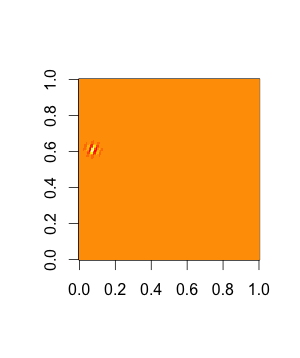
\includegraphics[width=\linewidth, height = 150pts]{voxel1_wave.png}
\endminipage\hfill
\vspace{-5mm}
\minipage{0.33\textwidth}
  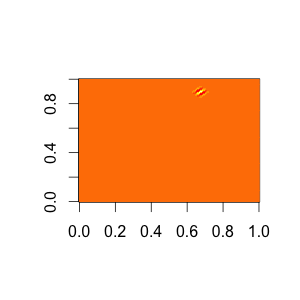
\includegraphics[width=\linewidth, height = 150pts]{voxel1_wave1.png}
\endminipage\hfill
\minipage{0.33\textwidth}
  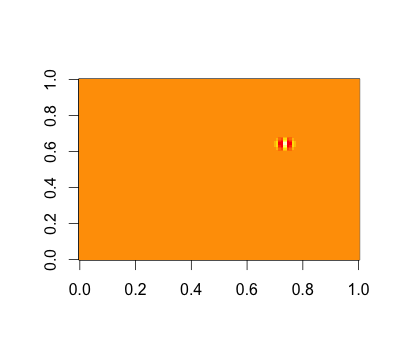
\includegraphics[width=\linewidth, height = 150pts]{voxel1_wave2.png}
\endminipage
  \caption{Voxel 1}\
\end{figure}
\vspace{-10mm}
\begin{figure}[H]
\minipage{0.33\textwidth}
  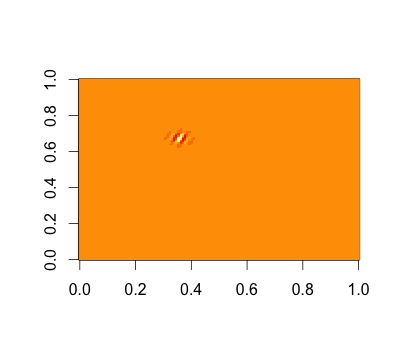
\includegraphics[width=\linewidth, height = 150pts]{voxel1_wave3.png}
\endminipage\hfill
\vspace{-5mm}
\minipage{0.33\textwidth}
  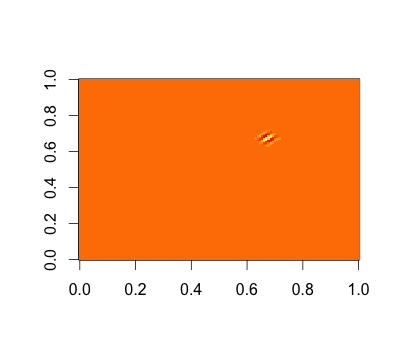
\includegraphics[width=\linewidth, height = 150pts]{voxel1_wave5.png}
\endminipage\hfill
\minipage{0.33\textwidth}
  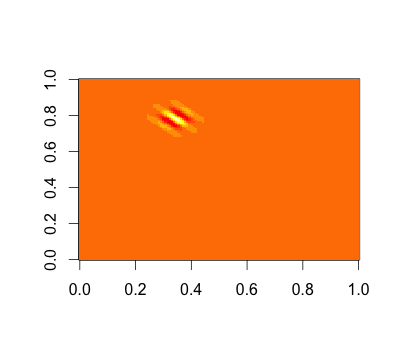
\includegraphics[width=\linewidth, height = 150pts]{voxel1_wave7.png}
\endminipage
  \caption{Voxel 1}
\end{figure}

\vspace{-10mm}
\begin{figure}[H]
\minipage{0.33\textwidth}
  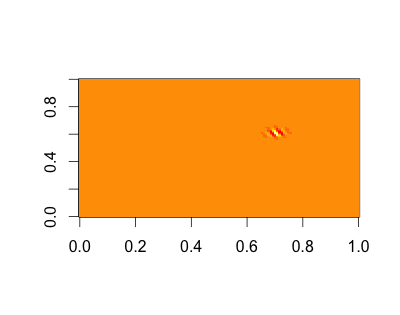
\includegraphics[width=\linewidth, height = 150pts]{voxel10_wave3.png}
\endminipage\hfill
\vspace{-5mm}
\minipage{0.33\textwidth}
  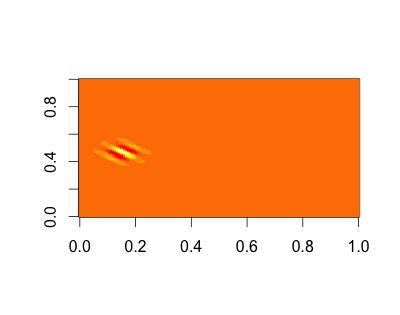
\includegraphics[width=\linewidth, height = 150pts]{voxel10_wave2.png}
\endminipage\hfill
\minipage{0.33\textwidth}
  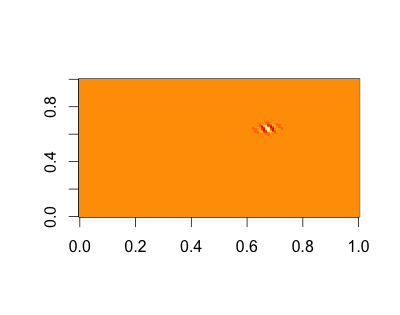
\includegraphics[width=\linewidth, height = 150pts]{voxel10_wave1.png}
\endminipage
  \caption{Voxel 10}
\end{figure}



\section{Conclusion}

In this lab, we were guided by the scientific question of how the brain processes visual data.  The dataset belonged to the regime of high dimensional problems, and many feature selection methods were used to optimize for both goals of predictability and interpretability.  Though random forest performed better in terms of the former goal, LASSO came out on top as achieving a balance of the two.  The penalty chosen and prediction error were stable against changes in (most) voxels, number of cross validation folds and size of the test set.  The predictions produced by the LASSO model captured the correlation structure of the original 20 voxels, though with lighter intensity.  This model also helped us derive some interpretive analysis of the features most important to voxels 1 and 10. \\




\section{Appendix 1}

The correlations between predicted voxel responses and actual voxel responses in the Lambda.min LASSO model are provided below, with 2 significant digits. 

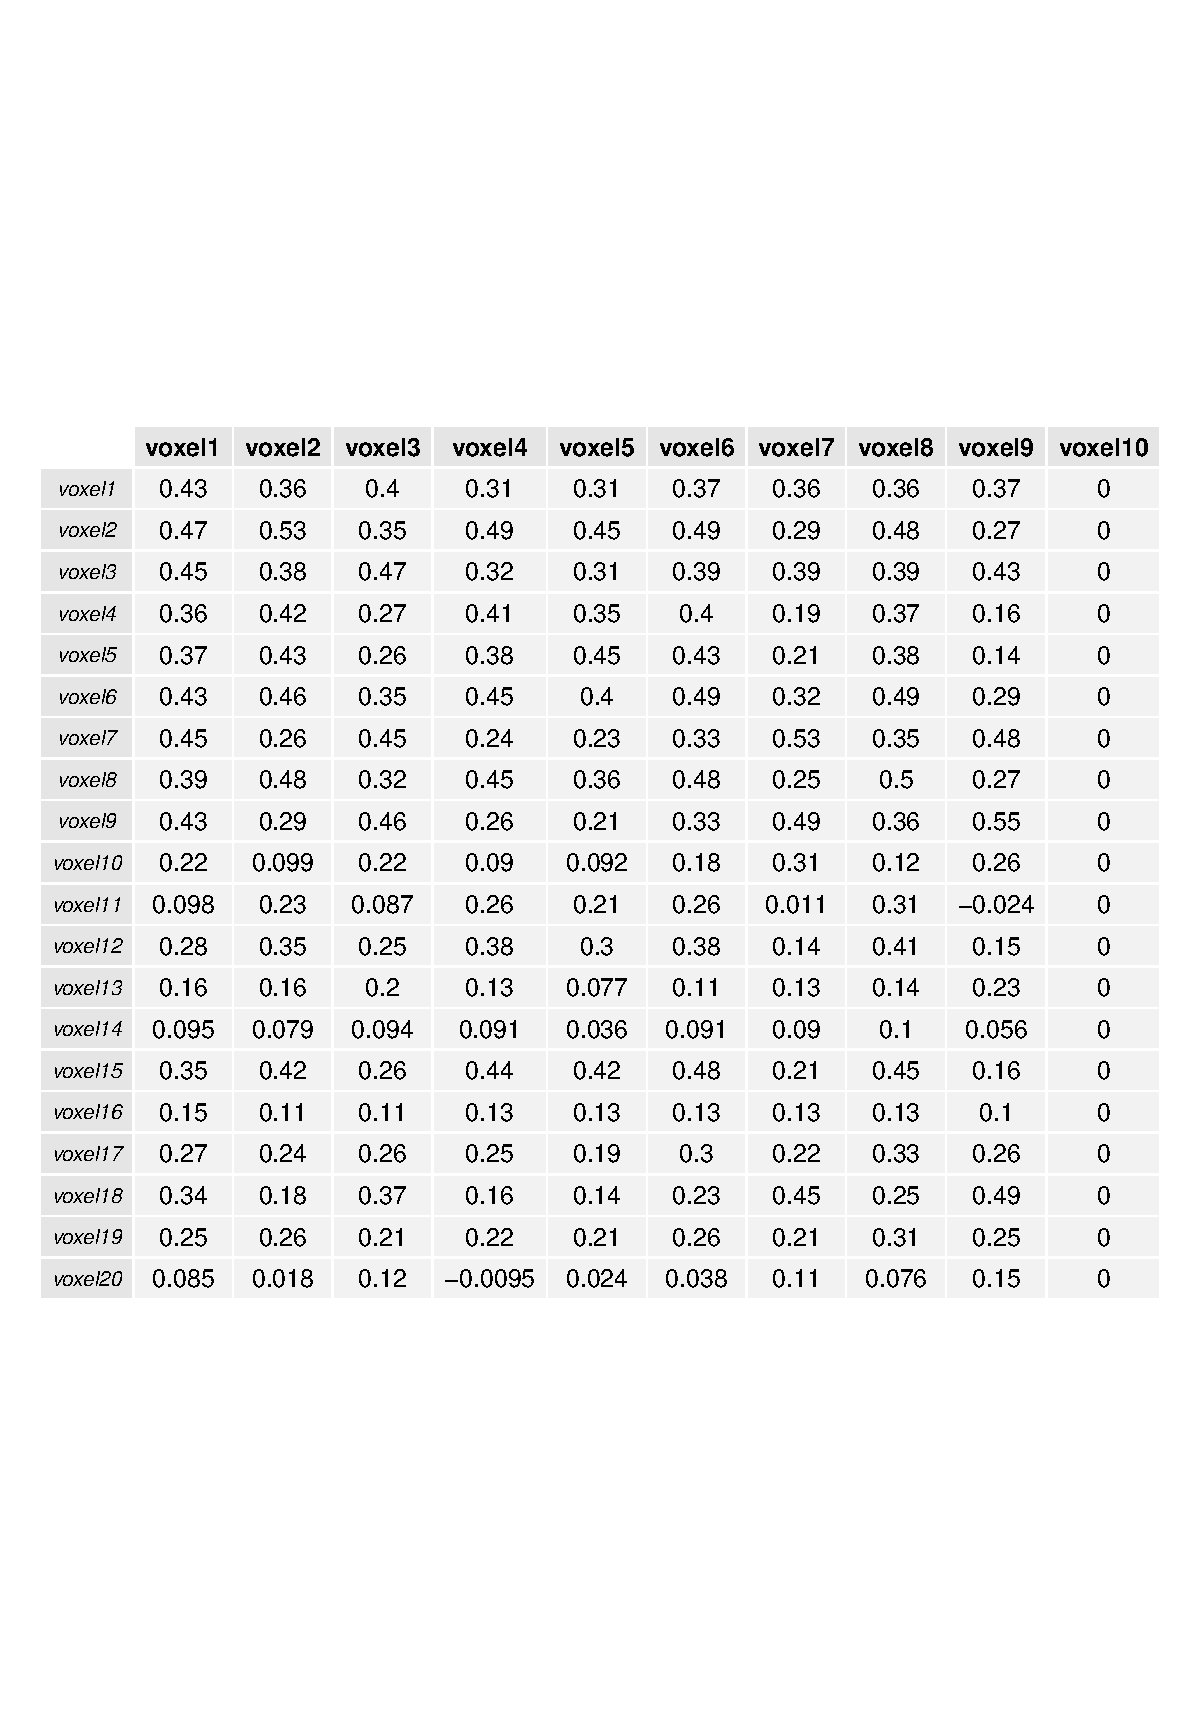
\includegraphics[width=\linewidth]{Corr_table2.pdf}
\newpage
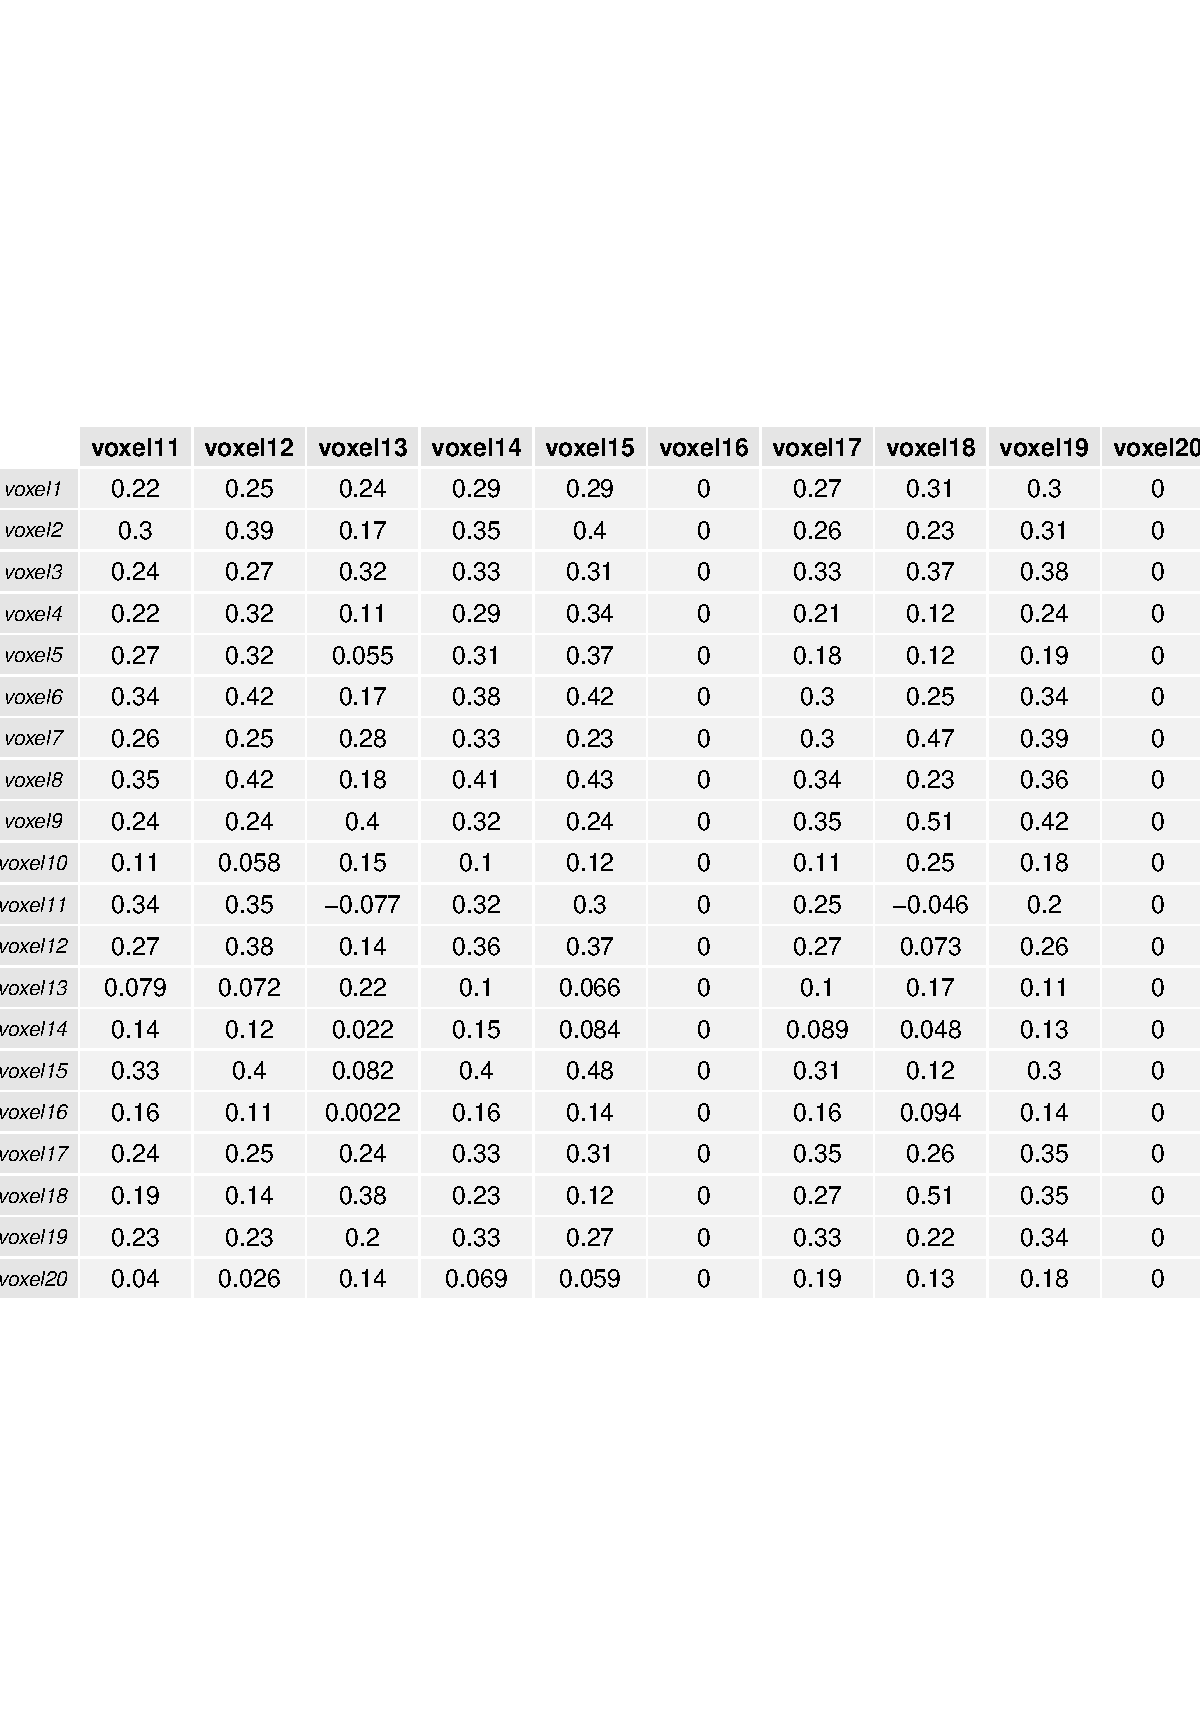
\includegraphics[width=\linewidth]{Corr_table1.pdf}

\end{document}
